\documentclass{article}

  % packages
    % basic stuff for rendering math
    \usepackage[letterpaper, top=1in, bottom=1in, left=1in, right=1in]{geometry}
    \usepackage[utf8]{inputenc}
    \usepackage[english]{babel}
    \usepackage{amsmath} 
    \usepackage{amssymb}
    % \usepackage{amsthm}

    % extra math symbols and utilities
    \usepackage{mathtools}        % for extra stuff like \coloneqq
    \usepackage{mathrsfs}         % for extra stuff like \mathsrc{}
    \usepackage{centernot}        % for the centernot arrow 
    \usepackage{bm}               % for better boldsymbol/mathbf 
    \usepackage{enumitem}         % better control over enumerate, itemize
    \usepackage{hyperref}         % for hypertext linking
    \usepackage{fancyvrb}          % for better verbatim environments
    \usepackage{newverbs}         % for texttt{}
    \usepackage{xcolor}           % for colored text 
    \usepackage{listings}         % to include code
    \usepackage{lstautogobble}    % helper package for code
    \usepackage{parcolumns}       % for side by side columns for two column code
    

    % page layout
    \usepackage{fancyhdr}         % for headers and footers 
    \usepackage{lastpage}         % to include last page number in footer 
    \usepackage{parskip}          % for no indentation and space between paragraphs    
    \usepackage[T1]{fontenc}      % to include \textbackslash
    \usepackage{footnote}
    \usepackage{etoolbox}

    % for custom environments
    \usepackage{tcolorbox}        % for better colored boxes in custom environments
    \tcbuselibrary{breakable}     % to allow tcolorboxes to break across pages

    % figures
    \usepackage{pgfplots}
    \pgfplotsset{compat=1.18}
    \usepackage{float}            % for [H] figure placement
    \usepackage{tikz}
    \usepackage{tikz-cd}
    \usepackage{circuitikz}
    \usetikzlibrary{arrows}
    \usetikzlibrary{positioning}
    \usetikzlibrary{calc}
    \usepackage{graphicx}
    \usepackage{algorithmic}
    \usepackage{caption} 
    \usepackage{subcaption}
    \captionsetup{font=small}

    % for tabular stuff 
    \usepackage{dcolumn}

    \usepackage[nottoc]{tocbibind}
    \pdfsuppresswarningpagegroup=1
    \hfuzz=5.002pt                % ignore overfull hbox badness warnings below this limit

  % New and replaced operators
    \newcommand{\qed}{\hfill$\blacksquare$}     % I like QED squares to be black

  % Custom Environments
    \newtcolorbox[auto counter, number within=section]{question}[1][]
    {
      colframe = orange!25,
      colback  = orange!10,
      coltitle = orange!20!black,  
      breakable, 
      title = \textbf{Question \thetcbcounter ~(#1)}
    }

    \newtcolorbox[auto counter, number within=section]{theorem}[1][]
    {
      colframe = red!25,
      colback  = red!10,
      coltitle = red!20!black,  
      breakable, 
      title = \textbf{Theorem \thetcbcounter ~(#1)}
    } 
    \newtcolorbox[auto counter, number within=section]{proposition}[1][]
    {
      colframe = red!25,
      colback  = red!10,
      coltitle = red!20!black,  
      breakable, 
      title = \textbf{Proposition \thetcbcounter ~(#1)}
    } 
    \newtcolorbox[auto counter, number within=section]{corollary}[1][]
    {
      colframe = red!25,
      colback  = red!10,
      coltitle = red!20!black,  
      breakable, 
      title = \textbf{Corollary \thetcbcounter ~(#1)}
    } 
    \newtcolorbox[auto counter, number within=section]{proof}[1][]
    {
      colframe = orange!25,
      colback  = orange!10,
      coltitle = orange!20!black,  
      breakable, 
      title = \textbf{Proof. }
    } 
    \newtcolorbox[auto counter, number within=section]{definition}[1][]
    {
      colframe = yellow!25,
      colback  = yellow!10,
      coltitle = yellow!20!black,  
      breakable, 
      title = \textbf{Definition \thetcbcounter ~(#1)}
    } 
    \newtcolorbox[auto counter, number within=section]{example}[1][]
    {
      colframe = blue!25,
      colback  = blue!10,
      coltitle = blue!20!black,  
      breakable, 
      title = \textbf{Example \thetcbcounter ~(#1)}
    } 
    \newtcolorbox[auto counter, number within=section]{code}[1][]
    {
      colframe = green!25,
      colback  = green!10,
      coltitle = green!20!black,  
      breakable, 
      title = \textbf{Code \thetcbcounter ~(#1)}
    } 
    \newtcolorbox[auto counter, number within=section]{algo}[1][]
    {
      colframe = green!25,
      colback  = green!10,
      coltitle = green!20!black,  
      breakable, 
      title = \textbf{Algorithm \thetcbcounter ~(#1)}
    } 

    \BeforeBeginEnvironment{example}{\savenotes}
    \AfterEndEnvironment{example}{\spewnotes}
    \BeforeBeginEnvironment{lemma}{\savenotes}
    \AfterEndEnvironment{lemma}{\spewnotes}
    \BeforeBeginEnvironment{theorem}{\savenotes}
    \AfterEndEnvironment{theorem}{\spewnotes}
    \BeforeBeginEnvironment{corollary}{\savenotes}
    \AfterEndEnvironment{corollary}{\spewnotes}
    \BeforeBeginEnvironment{proposition}{\savenotes}
    \AfterEndEnvironment{proposition}{\spewnotes}
    \BeforeBeginEnvironment{definition}{\savenotes}
    \AfterEndEnvironment{definition}{\spewnotes}
    \BeforeBeginEnvironment{exercise}{\savenotes}
    \AfterEndEnvironment{exercise}{\spewnotes}
    \BeforeBeginEnvironment{proof}{\savenotes}
    \AfterEndEnvironment{proof}{\spewnotes}
    \BeforeBeginEnvironment{solution}{\savenotes}
    \AfterEndEnvironment{solution}{\spewnotes}
    \BeforeBeginEnvironment{question}{\savenotes}
    \AfterEndEnvironment{question}{\spewnotes}
    \BeforeBeginEnvironment{code}{\savenotes}
    \AfterEndEnvironment{code}{\spewnotes}
    \BeforeBeginEnvironment{algo}{\savenotes}
    \AfterEndEnvironment{algo}{\spewnotes}

    \definecolor{dkgreen}{rgb}{0,0.6,0}
    \definecolor{gray}{rgb}{0.5,0.5,0.5}
    \definecolor{mauve}{rgb}{0.58,0,0.82}
    \definecolor{darkblue}{rgb}{0,0,139}
    \definecolor{lightgray}{gray}{0.93}
    \renewcommand{\algorithmiccomment}[1]{\hfill$\triangleright$\textcolor{blue}{#1}}

    % default options for listings (for code)
    \lstset{
      autogobble,
      frame=ltbr,
      language=Python,
      aboveskip=3mm,
      belowskip=3mm,
      showstringspaces=false,
      columns=fullflexible,
      keepspaces=true,
      basicstyle={\small\ttfamily},
      numbers=left,
      firstnumber=1,                        % start line number at 1
      numberstyle=\tiny\color{gray},
      keywordstyle=\color{blue},
      commentstyle=\color{dkgreen},
      stringstyle=\color{mauve},
      backgroundcolor=\color{lightgray}, 
      breaklines=true,                      % break lines
      breakatwhitespace=true,
      tabsize=3, 
      xleftmargin=2em, 
      framexleftmargin=1.5em, 
      stepnumber=1
    }

  % Page style
    \pagestyle{fancy}
    \fancyhead[L]{Python}
    \fancyhead[C]{Muchang Bahng}
    \fancyhead[R]{Fall 2024} 
    \fancyfoot[C]{\thepage / \pageref{LastPage}}
    \renewcommand{\footrulewidth}{0.4pt}          % the footer line should be 0.4pt wide
    \renewcommand{\thispagestyle}[1]{}  % needed to include headers in title page

\begin{document}

\title{Python}
\author{Muchang Bahng}
\date{Fall 2024}

\maketitle
\tableofcontents
\pagebreak

% To do 
% What is typing? How is Python type-checked?  
% Module symbol table  
% Try Except Finally  
% garbage collection: CPython currently uses a reference-counting scheme with (optional) delayed detection of cyclically linked garbage, which collects most objects as soon as they become unreachable, but is not guaranteed to collect garbage containing circular references. See the documentation of the gc module for information on controlling the collection of cyclic garbage. Other implementations act differently and CPython may change. Do not depend on immediate finalization of objects when they become unreachable (so you should always close files explicitly).

This covers computability theory, complexity theory, and automata theory. 
Alphabet. Boolean logic


\section{Lexical Analysis} 

  When we have code in a \texttt{.py} file and run it, the \textbf{lexical analyzer} generates a stream of \textbf{tokens} to be inputted into a parser. 

  \begin{theorem}
    All UTF-8 characters can be parsed by the lexical analyzer. 
  \end{theorem}

  \begin{question}
    Which characters aren't? 
  \end{question}

  \begin{definition}[Logical and Physical Lines] 
    There are two types of lines in Python. 
    \begin{enumerate}
      \item A \textbf{logical line} is represented by the token \texttt{NEWLINE}. 
      \item A \textbf{physical line} is a sequence of characters terminated by an end-of-line (EOL) sequence. 
    \end{enumerate} 
    \begin{lstlisting}
      x = [1, 2, 3, 4]  # one logical line on one physical line 
      x = [1, 2,        # one logical line on two physical lines
           3, 4]
    \end{lstlisting}
  \end{definition} 

\section{Types} 

  The development of the Python type hierarchy is a bit involved and requires you to know both implementation details and history. During the early days of Python 2, the language had both \textit{types} and \textit{classes}. Types were built-in objects implemented in C, and classes were what you built when using a \texttt{class} statement. These two were named differently because you couldn't mix these; classes could not extend types. However, this difference was artificial and ultimately a limitation in the language implementation. Starting with Python 2.2, the developers of Python have slowly moved towards unifying the two concepts, which the difference completely done in Python 3. Built-in types are now labeled classes, and you can extend them at will. Since we are working in Python 3, they are interchangeable.  

  \begin{theorem}[Types and Classes]
    In Python 3, types and classes mean the same thing. 
  \end{theorem} 

  Let's do a bit of review on classes. 

  \begin{definition}[Class] 
    A \textbf{class} is a template for creating objects, which support \textit{attributes} to store some state and \textit{methods} that may or may not modify the state. The object that is created from a class is called a \textbf{class instance}. 

    \begin{lstlisting}
      class ClassName: 
        ...  
    \end{lstlisting}
  \end{definition}

  \begin{example}[Animal Class Definition]
    A class can be instantiated with the following. 

    \begin{figure}[H]
      \centering 
      \begin{lstlisting}
        class Animal: 
            def __init__(self, name):
                self.name = name
            
            def speak(self):
                return f"{self.name} makes a sound"
      \end{lstlisting} 
      \caption{} 
      \label{fig:animal_class}
    \end{figure}
  \end{example}  

\subsection{Dunder Methods}

  It is important to have good tools to analyze the class itself and the instance. These are mainly stored in \textit{dunder (double underscore)} methods, also called \textit{magic methods}. 

  \begin{definition}[Class and Type Information]
    \begin{table}[H]
      \centering
      \begin{tabular}{|c|p{8cm}|}
        \hline
        \textbf{Functions} & \textbf{Description} \\
        \hline 
        \texttt{hasattr(obj, "attr\_name")} & checks if an object has a specific attribute \\
        \hline
        \texttt{isinstance(obj, ClassA)} & checks if an object is an instance of a class \\
        \hline
        \texttt{issubclass(ClassA, ClassB)} & checks if one class is a subclass of another \\
        \hline
        \texttt{type(obj)} & returns the type/class of an object \\
        \hline
        \texttt{dir(obj)} & lists all attributes and methods of an object \\
        \hline
        \texttt{vars(obj)} & returns the \_\_dict\_\_ of an object \\
        \hline
        \texttt{obj.\_\_dict\_\_} & dictionary containing the object's attributes \\
        \hline
        \texttt{obj.\_\_class\_\_} & reference to the object's class \\
        \hline
        \texttt{ClassA.\_\_name\_\_} & name of the class \\
        \hline
        \texttt{ClassA.\_\_module\_\_} & module where the class was defined \\
        \hline
        \texttt{ClassA.\_\_bases\_\_} & tuple of base classes \\
        \hline
        \texttt{ClassA.\_\_mro\_\_} & method resolution order tuple \\
        \hline
        \texttt{\_\_getattr\_\_(self, name)} & called when attribute doesn't exist \\
        \hline
        \texttt{\_\_setattr\_\_(self, name, value)} & called when setting attributes \\
        \hline
        \texttt{\_\_delattr\_\_(self, name)} & called when deleting attributes \\
        \hline
        \texttt{\_\_getattribute\_\_(self, name)} & called for all attribute access \\
        \hline
      \end{tabular}
      \caption{Class instances (objects) are marked with \texttt{obj} and Class definitions with \texttt{ClassA}.}
      \label{tab:functions_for_classes}
    \end{table}
  \end{definition}

  \begin{definition}[Documentation and Metadata]
    \begin{table}[H]
      \centering
      \begin{tabular}{|c|p{8cm}|}
        \hline
        \textbf{Attributes} & \textbf{Description} \\
        \hline 
        \texttt{obj.\_\_doc\_\_} & docstring of the class or method \\
        \hline
        \texttt{obj.\_\_annotations\_\_} & type annotations dictionary \\
        \hline
      \end{tabular}
      \caption{Documentation and metadata attributes for classes and objects.}
      \label{tab:documentation_metadata}
    \end{table}
  \end{definition}

  \begin{definition}[Object Lifecycle]
    \begin{table}[H]
      \centering
      \begin{tabular}{|c|p{8cm}|}
        \hline
        \textbf{Methods} & \textbf{Description} \\
        \hline 
        \texttt{\_\_init\_\_(self, ...)} & constructor method \\
        \hline
        \texttt{\_\_new\_\_(cls, ...)} & object creation method (called before \_\_init\_\_) \\
        \hline
        \texttt{\_\_del\_\_(self)} & destructor method \\
        \hline
      \end{tabular}
      \caption{Methods that control object creation and destruction.}
      \label{tab:object_lifecycle}
    \end{table}
  \end{definition}

  \begin{definition}[String Representation]
    \begin{table}[H]
      \centering
      \begin{tabular}{|c|p{8cm}|}
        \hline
        \textbf{Methods} & \textbf{Description} \\
        \hline 
        \texttt{\_\_str\_\_(self)} & informal string representation (used by str()) \\
        \hline
        \texttt{\_\_repr\_\_(self)} & official string representation (used by repr()) \\
        \hline
      \end{tabular}
      \caption{Methods for string representation of objects.}
      \label{tab:string_representation}
    \end{table}
  \end{definition}

  \begin{definition}[Comparison and Hashing]
    \begin{table}[H]
      \centering
      \begin{tabular}{|c|p{8cm}|}
        \hline
        \textbf{Methods} & \textbf{Description} \\
        \hline 
        \texttt{\_\_eq\_\_(self, other)} & equality comparison (==) \\
        \hline
        \texttt{\_\_lt\_\_(self, other)} & less than comparison (<) \\
        \hline
        \texttt{\_\_gt\_\_(self, other)} & greater than comparison (>) \\
        \hline
        \texttt{\_\_le\_\_(self, other)} & less than or equal (<=) \\
        \hline
        \texttt{\_\_ge\_\_(self, other)} & greater than or equal (>=) \\
        \hline
        \texttt{\_\_ne\_\_(self, other)} & not equal (!=) \\
        \hline
        \texttt{\_\_hash\_\_(self)} & hash value for the object \\
        \hline
      \end{tabular}
      \caption{Methods for object comparison and hashing.}
      \label{tab:comparison_hashing}
    \end{table}
  \end{definition}

  \begin{definition}[Container-like Behavior]
    \begin{table}[H]
      \centering
      \begin{tabular}{|c|p{8cm}|}
        \hline
        \textbf{Methods} & \textbf{Description} \\
        \hline 
        \texttt{\_\_len\_\_(self)} & length of the object \\
        \hline
        \texttt{\_\_getitem\_\_(self, key)} & get item by index/key (obj[key]) \\
        \hline
        \texttt{\_\_setitem\_\_(self, key, value)} & set item by index/key (obj[key] = value) \\
        \hline
        \texttt{\_\_delitem\_\_(self, key)} & delete item by index/key (del obj[key]) \\
        \hline
        \texttt{\_\_iter\_\_(self)} & makes object iterable \\
        \hline
        \texttt{\_\_contains\_\_(self, item)} & supports 'in' operator \\
        \hline
      \end{tabular}
      \caption{Methods that make objects behave like containers.}
      \label{tab:container_behavior}
    \end{table}
  \end{definition}

  \begin{definition}[Mathematical Operations] 
    Most of the math operators in Python (\texttt{+}, \texttt{-}, ...) actually call some dunder method. We can define these dunder methods in order to use mathematical operations on class objects, e.g. \texttt{a + b}. 

    \begin{table}[H]
      \centering
      \begin{tabular}{|c|p{8cm}|}
        \hline
        \textbf{Methods} & \textbf{Description} \\
        \hline 
        \texttt{\_\_add\_\_(self, other)} & called when we evaluate \texttt{self + other} \\
        \hline
        \texttt{\_\_sub\_\_(self, other)} & called when we evaluate \texttt{self - other} \\
        \hline
        \texttt{\_\_mul\_\_(self, other)} & called when we evaluate \texttt{self * other} \\
        \hline
        \texttt{\_\_truediv\_\_(self, other)} & called when we evaluate \texttt{self / other} \\
        \hline
        \texttt{\_\_floordiv\_\_(self, other)} & called when we evaluate \texttt{self // other} \\
        \hline
        \texttt{\_\_mod\_\_(self, other)} & called when we evaluate \texttt{self \% other} \\
        \hline
        \texttt{\_\_pow\_\_(self, other)} & called when we evaluate \texttt{self ** other} \\
        \hline
        \texttt{\_\_and\_\_(self, other)} & called when we evaluate \texttt{self \& other} \\
        \hline
        \texttt{\_\_or\_\_(self, other)} & called when we evaluate \texttt{self | other} \\
        \hline
        \texttt{\_\_xor\_\_(self, other)} & called when we evaluate \texttt{self \^{} other} \\
        \hline
        \texttt{\_\_lshift\_\_(self, other)} & called when we evaluate \texttt{self << other} \\
        \hline
        \texttt{\_\_rshift\_\_(self, other)} & called when we evaluate \texttt{self >> other} \\
        \hline
        \texttt{\_\_neg\_\_(self)} & called when we evaluate \texttt{-self} \\
        \hline
        \texttt{\_\_pos\_\_(self)} & called when we evaluate \texttt{+self} \\
        \hline
        \texttt{\_\_abs\_\_(self)} & called when we evaluate \texttt{abs(self)} \\
        \hline
        \texttt{\_\_invert\_\_(self)} & called when we evaluate \texttt{\~{}self} \\
        \hline
        \texttt{\_\_round\_\_(self, ndigits)} & called when we evaluate \texttt{round(self)} \\
        \hline
        \texttt{\_\_floor\_\_(self)} & called when we evaluate \texttt{math.floor(self)} \\
        \hline
        \texttt{\_\_ceil\_\_(self)} & called when we evaluate \texttt{math.ceil(self)} \\
        \hline
        \texttt{\_\_trunc\_\_(self)} & called when we evaluate \texttt{math.trunc(self)} \\
        \hline
      \end{tabular}
      \caption{Methods for mathematical operations on objects.}
      \label{tab:mathematical_operations}
    \end{table}

    Note that in the abstract algebraic sense, \texttt{a + b} is really just a binary operation and may not be commutative. There are also \textit{reverse versions} of the binary operations, e.g. \texttt{\_\_radd\_\_}, that are called when the left operand doesn't support the operation. There are also \textit{in-place versions} like \texttt{\_\_iadd\_\_()} for operations like \texttt{+=}.  
  \end{definition}

\subsection{Encapsulation} 

  
 
\subsection{Inheritance and Method Resolution Order} 

  Conceptually, we might think of certain types a subset of another type. Therefore, it makes sense to design some \textit{hierarchy} of these types where children can extend the functionality of their parents. This is the conceptual idea of inheritance, which is a convenient way of designing code. In fact, if we had infinite coding power where we don't care about maintainability or the DRY (don't repeat yourself) principle, then you wouldn't need inheritance. 

  \begin{definition}[Class Inheritance]
    A \textbf{child class} can inherit the attributes and methods of the parent class, and in general should \textit{extend} the functionality of the base class. Here is the minimal example. 

    \begin{figure}[H]
      \centering
      \begin{subfigure}[b]{0.48\textwidth}
        \centering
        \begin{lstlisting}
          class P: 
            ... 
          class B(A): 
            ...
        \end{lstlisting}
        \caption{Inheritance with 1 parent class and 1 child class.}
      \end{subfigure}
      \hfill 
      \begin{subfigure}[b]{0.48\textwidth}
        \centering
        \begin{lstlisting}
          class P1: ... 
          class P2: ...
          class P3: ... 
          class C(P1, P2, P3): ...
        \end{lstlisting}
        \caption{Multiple inheritance with 3 parent and 1 child class.}
      \end{subfigure}
      \caption{}
    \end{figure}
  \end{definition}


  A more directly practical advantage of coding is that we can take advantage of the \textit{method resolution order (MRO)}. Let's introduce what this is slowly with a sequence of examples. 

  \begin{example}[Methods of Parent are Accessible from Child]
    Consider the two classes. 
    \begin{lstlisting}
      class Animal: 
        def __init__(self, name): 
          self.name = name 

        def speak(self): 
          print("Rah") # generic animal sound

      class Dog(Animal): 
        ...
    \end{lstlisting} 
    The only way \texttt{Dog} is connected to \texttt{Animal} is that it is declared as a subclass of \texttt{Animal}. It may not look like \texttt{Dog} even has a constructor method, but in fact we can access both the \texttt{\_\_init\_\_} and \texttt{speak} methods! 
    \begin{lstlisting} 
      >>> x = Dog("wolfy") 
      >>> x.speak() 
      "Rah"
    \end{lstlisting}
  \end{example} 

  So we have found out that subclasses can access parent class methods by default. But what if we have \textit{multiple} parent classes?  

  \begin{example}[Method Resolution with Multiple Parent Classes]
    Say that we have the same \texttt{Animal} class as defined above, but with the following hierarchy. 

    \begin{figure}[H]
      \centering
      \begin{subfigure}[b]{0.48\textwidth}
        \centering
        \begin{lstlisting}
          class Animal: 
            def __init__(self, name):
              print("Animal constructor called.")
              self.name = name
            
            def speak(self):
              return f"{self.name} makes a sound"  

          class Flyer(Animal):  
            def __init__(self, name): 
              print("Flyer constructor called") 

          class Swimmer(Animal): 
            def __init__(self, name): 
              print("Swimmer constructor called") 
        \end{lstlisting}
        \caption{}
      \end{subfigure}
      \hfill 
      \begin{subfigure}[b]{0.48\textwidth}
        \centering
        \begin{lstlisting}
          class Duck1(Flyer, Swimmer): 
            ... 

          class Duck2(Swimmer, Flyer): 
            ...

          class Duck3(Flyer, Swimmer): 
            def __init__(self, name): 
              print("Duck constructor called")
        \end{lstlisting}
        \caption{}
      \end{subfigure}
      \caption{}
    \end{figure}

    Interesting, so it seems like if the child class supports its own constructor, then it will call its own constructor, and if not, then it will look at the constructors of the parent classes, \textit{in the order in which they were specified} when defining the child class. 
      
    \begin{lstlisting}
      >>> Duck1("duck1")
      Flyer constructor called
      >>> Duck2("duck2")
      Swimmer constructor called
      >>> Duck3("duck3")
      Duck constructor called
    \end{lstlisting} 
  \end{example} 

  So when a subclass is instantiated, the child class somehow knows where to look first for an implementation of a method to call, then next, then next, etc. This ordering is extremely useful, though can be a double-edged sword.   

  \begin{definition}[Method Resolution Order]
    The \textbf{method resolution order (MRO)} of a given class \texttt{C} is a sequence of classes that Python looks through to find an implementation of any method. 
    \begin{enumerate}
      \item It is a tuple that can be retrieved with \texttt{C.\_\_mro\_\_} (this is a class method). 
      \item The actual way that the MRO is computed is with the \href{https://docs.python.org/3/howto/mro.html}{C3 Algorithm}, starting from Python 2.3.
    \end{enumerate}
  \end{definition}

  \begin{example}[MROs of Ducks]
    The MROs of the Duck classes confirms our suspicion. Generally, we go from the most specific class to the broadest class, which is always \texttt{object} in Python. 

    \begin{lstlisting}
      >>> print(Duck1.__mro__)
      (<class '__main__.Duck1'>, <class '__main__.Flyer'>, <class '__main__.Swimmer'>, <class '__main__.Animal'>, <class 'object'>)

      >>> print(Duck2.__mro__)
      (<class '__main__.Duck2'>, <class '__main__.Swimmer'>, <class '__main__.Flyer'>, <class '__main__.Animal'>, <class 'object'>)

      >>> print(Duck3.__mro__)
      (<class '__main__.Duck3'>, <class '__main__.Flyer'>, <class '__main__.Swimmer'>, <class '__main__.Animal'>, <class 'object'>)
    \end{lstlisting}
  \end{example} 

  In most cases, when you are trying to call a method from a parent class, you are most likely trying to find the next class in the MRO that implements this method, which may not be the direct parent.\footnote{\href{https://stackoverflow.com/questions/222877/what-does-super-do-in-python-difference-between-super-init-and-expl}{https://stackoverflow.com/questions/222877/what-does-super-do-in-python-difference-between-super-init-and-expl}}. So rather than explicitly hard-coding something like this 

  \begin{lstlisting}
    class P: 
      def method(self): 
        ...

    class C(P): 
      def method(self): 
        P.method(self) 
        ...
  \end{lstlisting} 

  You might have heard that you should use something called \texttt{super()}. 

  \begin{definition}[Superclass] 
    The \textbf{superclass \texttt{S} with respect to a method \texttt{m}} of a class \texttt{C} is the next class in the MRO that actually implements the method \texttt{m}. This can be gotten by calling \texttt{super()}.\footnote{Note that unlike other sources, I distinguish the superclass and the parent class. The superclass is with respect to a method, and the parent class does not need to specify a method.}
  \end{definition} 

  The MRO is useful when calling methods not explicitly defined in our child class (but defined in some parent class), but ultimately, the whole point of having child classes is so that we can \textit{extend} our parent classes. For example, the first thing we must always do with an object is to instantiate it---through the constructor. There are three general ways that we can implement the constructor of child class \texttt{C} with parent class \texttt{P}. 

  \begin{enumerate}
    \item Do not define the constructor on \texttt{C}. Then, the MRO will just call the constructor of the parent class. 

    \begin{figure}[H]
      \centering
      \begin{subfigure}[b]{0.48\textwidth}
        \centering
        \begin{lstlisting}
          class P: 
            def __init__(self, name): 
              self.name = name
        \end{lstlisting}
        \caption{}
      \end{subfigure}
      \hfill 
      \begin{subfigure}[b]{0.48\textwidth}
        \centering
        \begin{lstlisting}
          class C(P): 
            ...
            .
        \end{lstlisting}
        \caption{}
      \end{subfigure}
      \caption{}
    \end{figure}

    \item Define the constructor on \texttt{C}, but do not call the parent's constructor. This allows you to completely override the parent constructor, but this is a bad idea for two reasons. First, if you are really just re-implementing the same thing that the parent constructor has done, then you are better off doing (3). If you truly need to override the \textit{whole} parent constructor, then perhaps you are not truly extending the parent class, and class inheritance is not the right approach. 

    \begin{figure}[H]
      \centering
      \begin{subfigure}[b]{0.48\textwidth}
        \centering
        \begin{lstlisting}
          class P: 
            def __init__(self, name): 
              self.name = name
          .
        \end{lstlisting}
        \caption{}
      \end{subfigure}
      \hfill 
      \begin{subfigure}[b]{0.48\textwidth}
        \centering
        \begin{lstlisting}
          class C(P): 
            def __init__(self, name, breed): 
              self.name = name 
              self.breed = breed
        \end{lstlisting}
        \caption{}
      \end{subfigure}
      \caption{}
    \end{figure}

    \item Define the constructor on \texttt{C}. In the child constructor, call the parent's constructor to set up all of the parent's attributes, and then add your own or do some postprocessing after. 

    \begin{figure}[H]
      \centering
      \begin{subfigure}[b]{0.48\textwidth}
        \centering
        \begin{lstlisting}
          class P: 
            def __init__(self, name): 
              self.name = name
          .
        \end{lstlisting}
        \caption{}
      \end{subfigure}
      \hfill 
      \begin{subfigure}[b]{0.48\textwidth}
        \centering
        \begin{lstlisting}
          class C(P): 
            def __init__(self, name, breed): 
              super().__init__(name)
              self.breed = breed
        \end{lstlisting}
        \caption{}
      \end{subfigure}
      \caption{}
    \end{figure}
  \end{enumerate}

  It's clear what the best choice is. Since we generally want to retain the class attributes (hence call parent constructor) and extend them (hence explicitly define the child constructor), we should by default opt for the third choice. 

  \begin{theorem}[Heuristic]
    In the beginning of your child constructor, you should almost always call \texttt{super().\_\_init\_\_(*args)}. 
  \end{theorem} 

  You might also notice that not implementing a constructor method at all is equivalent to just implementing a constructor method with only \texttt{super().\_\_init\_\_()}.\footnote{\href{https://stackoverflow.com/questions/61174178/why-is-python-super-used-in-the-childs-init-method}{https://stackoverflow.com/questions/61174178/why-is-python-super-used-in-the-childs-init-method}}. However, this is still bad for maintainability, and can be especially dangerous if there are keyword arguments that are passed on. 

  For the constructor, we've seen that we must always define \texttt{\_\_init\_\_()} and have it call the super's constructor. This generally comes from the fact that the attributes of a child class should be a strict superset of those of parent classes. For methods, we may either want a method \texttt{m()} of a child class to call super's method as well, along with doing additional things, or we might want to completely override it. Consider the animal class again. 
  \begin{lstlisting}
    class Animal: 
      def __init__(self, name):
        self.name = name
      
      def speak(self):
        return f"Rahhh" # generic animal sound
  \end{lstlisting} 

  Overriding and extending methods is straightforward. 

  \begin{figure}[H]
    \centering
    \begin{subfigure}[b]{0.48\textwidth}
      \centering
      \begin{lstlisting}
        class Dog(Animal): 
          def speak(self): 
            return "woof"
        .
      \end{lstlisting}
      \caption{To override, just redefine it, and the MRO will view this implementation first.}
    \end{subfigure}
    \hfill 
    \begin{subfigure}[b]{0.48\textwidth}
      \centering
      \begin{lstlisting}
        class Dog(Animal): 
          def speak(self): 
            return super().speak() + " said the dog."
      \end{lstlisting}
      \caption{To extend it, have it call the super's method first, and then do whatever you want after. }
    \end{subfigure}
    \caption{}
  \end{figure}

  Deleting any parent attribute or method is not a good idea and goes against the whole purpose of inheritance. If it must be done, here are the best methods I know. 

  \begin{theorem}[Deleting Attribute Belonging to Parent in Child]
    You can delete an attribute from the child class by calling \texttt{delattr(ChildClass, "attribute")}. 
    \begin{lstlisting}
      class P: 
        def __init__(self, name): 
          self.name = name  

      class C(P): 
        def __init__(self, name): 
          super().__init__(self, name) 
          delattr(C, "name") 
    \end{lstlisting}
  \end{theorem}

  \begin{theorem}[Deleting Method Belong to Parent in Child]
    You cannot delete a method that exists in the parent class from the child class, since the MRO will just be invoked. The best you can do is override it to throw an exception. 
  \end{theorem}

  \begin{example}[Modifying Attributes in Child Class]
    We begin with an \texttt{Animal} class.

    \begin{figure}[H]
      \centering 
      \begin{lstlisting}
        class Animal: 
            def __init__(self, name):
                self.name = name
            
            def speak(self):
                return f"Rahhh" # generic animal sound
      \end{lstlisting} 
      \caption{} 
    \end{figure}

    There is a \texttt{Dog} class that we would like to inherit from \texttt{Animal}. Let's go through a few ways we can design the attributes of the child class. 

    \begin{figure}[H]
      \centering
      \begin{subfigure}[b]{0.48\textwidth}
        \centering
        \begin{lstlisting}
          class Dog(Animal): 
            def __init__(self, name): 
              super().__init__(name) 
          .
        \end{lstlisting}
        \caption{Nothing is added. Since called the parent constructor, we still have access to the \texttt{name} attribute and \texttt{speak} method. }
      \end{subfigure}
      \hfill 
      \begin{subfigure}[b]{0.48\textwidth}
        \centering
        \begin{lstlisting}
          class Dog(Animal): 
            def __init__(self, name, breed): 
              super().__init__(name)
              self.breed = breed
        \end{lstlisting}
        \caption{We just want to add a new attribute called \texttt{breed}. Since called the parent constructor, we still have access to the \texttt{name} attribute and \texttt{speak} method. }
      \end{subfigure}

      \begin{subfigure}[b]{0.48\textwidth}
        \centering
        \begin{lstlisting}
          class Dog(Animal): 
            def __init__(self, id): 
              self.id = id
        \end{lstlisting}
        \caption{You don't even call the parent constructor, so you lose access to \texttt{name}. However, you still have access to the \texttt{speak()} method. This is not recommended.}
      \end{subfigure}
      \hfill 
      \begin{subfigure}[b]{0.48\textwidth}
        \centering
        \begin{lstlisting}
          class Dog(Animal): 
            def __init__(self, name, breed): 
              super().__init__(name)  
              print(self.name)
              self.name = f"{name}_{breed}"
        \end{lstlisting}
        \caption{Say you want to override the name so that the breed is also included in it.}
      \end{subfigure}
      \caption{}
    \end{figure}
  \end{example}

\subsection{Interfaces and Abstract Base Classes} 

  Note that inheritance does two things. First, it allows us to reuse code since a child class inherits attributes/methods from a superclass. Second, we can extend or override parent functionality, which allows us to use different implementations of the same method. The fancy sounding term ``polymorphism'' is just a colloqial buzzword that refers to being able to treat objects of different types in the same way, mostly through calling a method with the same name. 

  \begin{definition}[Polymorphism]
    \textbf{Polymorphism} is the ability of objects of different types to be treated as instances of the same type through a common interface. It comes in many forms, including 
    \begin{enumerate}
      \item \textit{Subtype/Inclusion Polymorphism}. Basically what we did with inheritance. 
      \item \textit{Parameteric Polymorphism}. Allows function or data type to be written generically, so that it can handle values \textit{uniformly} without depending on their type. 
      \item \textit{Overriding}. 
      \item \textit{Overloading}. Taking the 
    \end{enumerate}
  \end{definition}

  With inheritance, we can create hierarchies of classes where child classes extend or override parent functionality. However, we are still short 

  At this point, we have defined the class hierarchy by taking the class names (more specifically, the \textit{fully qualified class name (FQCN)}) and explicitly defining a parent-child relationship (e.g. \texttt{Dog(Animal)}). As stated in \href{https://peps.python.org/pep-3119/}{PEP-3119}, in the domain of OOP, the uage patterns of interacting with an object can be divided into two basic categories. 
  \begin{enumerate}
    \item \textit{Invocation}. Interacting with an object by invoking its methods. 
    \item \textit{Inspection}. The ability for external code (outside of the object's methods) to examine the type or properties of that object, and make decisions on how to treat that object based on that information. 
  \end{enumerate}
  Both usage patterns 

\subsection{Interfaces and Abstract Base Classes} 

  Apparently need to know for PEP 3119. 

  But classes are limited? So we want to use interfaces (duck typing). 

    % - Implemented as ABCs in python. 
    % - A new module abc which serves as an “ABC support framework”. It defines a metaclass for use with ABCs and a decorator that can be used to define abstract methods. 
    % - PEP 3141 gives a hierarchy of the numbers.  
    % - ABCs have two points, one obtained by subclassing ("invasive"), one by registering (non-invasive). (https://stackoverflow.com/questions/3392352/python-abcs-registering-vs-subclassing) 
    % 

  PEP 3141 gives a hierarchy of the numbers. 

  \begin{definition}[Numeric ABCs] 
    The \texttt{numbers} module contains them. 
    \begin{enumerate}
      \item \texttt{numbers.Number} 
      \item \texttt{numbers.Complex} 
      \item \texttt{numbers.Real} 
      \item \texttt{numbers.Rational} 
      \item \texttt{numbers.Integral} 
    \end{enumerate}
  \end{definition}

\subsection{Type Hints}

  Type Hints - PEP 484 (3.5) 

\subsection{Protocols}

  Protocols - PEP 544 (3.7) 

\subsection{Type Checking}

  \begin{question}[To Do]
    Move some of these to general language notes. 
  \end{question}

  \begin{definition}[Type Checking]
    \textbf{Type checking} is the process of verifying that the types of values in a program are used consistently and correctly according to the language's type system rules. These include: 
    \begin{enumerate}
      \item Operations are valid for their operand types 
      \item Function/method calls match their signatures 
      \item Assignments are type-compatible (though this isn't necessary in Python) 
    \end{enumerate}
  \end{definition}

  The implementation of type checking differs for every language, and they generally fall into 3 different philosophies. 

  \begin{definition}[Nominal Typing]
    \textbf{Nominal typing} is a static typing system that determines that two types are equal/compatible if their fully qualified class names (FQCN) are equal. 

    \begin{figure}[H]
      \centering 
      \noindent\begin{minipage}{.5\textwidth}
        \begin{lstlisting}[language=C++]{Code}
          struct Cat {
              std::string name;
              int age;
          };

          void printCat(const Cat& c) {
              std::cout << "Cat: " << c.name << ", age " << c.age << "\n";
          }        
        \end{lstlisting}
        \end{minipage}
        \hfill
        \begin{minipage}{.49\textwidth}
        \begin{lstlisting}[language=C++]{Output}
          struct Dog {
              std::string name;
              int age;
          };

          void printDog(const Dog& d) {
              std::cout << "Dog: " << d.name << ", age " << d.age << "\n";
          }
        \end{lstlisting}
      \end{minipage}

      \begin{lstlisting}[language=C++]
        int main() {
            Cat kitty{"Whiskers", 3};
            Dog pup{"Buddy", 5};

            printCat(kitty); // works
            printDog(pup);   // works

            // printCat(pup); // error: cannot convert Dog to Cat (nominal typing)

            return 0;
        } 
      \end{lstlisting}
      \caption{C++ uses aspects of nominal typing.} 
      \label{fig:cpp_nominal}
    \end{figure}
  \end{definition}

  \begin{definition}[Structural Typing]
    \textbf{Structural typing} is a static typing system that determines that two types are equal/compatible if their structures (e.g. the attributes and methods it supports) are equal. The class name is immaterial. 

    \begin{figure}[H]
      \centering 
      \noindent\begin{minipage}{.5\textwidth}
        \begin{lstlisting}[language=php]{Code}
          type Cat = {
            name: string;
            age: number;
          };

          function printCat(c: Cat) {
            console.log(`Cat: ${c.name}, age ${c.age}`);
          }
        \end{lstlisting}
        \end{minipage}
        \hfill
        \begin{minipage}{.49\textwidth}
        \begin{lstlisting}[]{Output}
          type Dog = {
            name: string;
            age: number;
          };

          function printDog(d: Dog) {
            console.log(`Dog: ${d.name}, age ${d.age}`);
          }
        \end{lstlisting}
      \end{minipage}

      \begin{lstlisting}
        const kitty: Cat = { name: "Whiskers", age: 3 };
        const pup: Dog = { name: "Buddy", age: 5 };

        printCat(kitty); // works
        printDog(pup);   // works
        printCat(pup);   // also works (structural typing!)
      \end{lstlisting}
      \caption{Typescript uses aspects of structural typing.} 
      \label{fig:typescript_structural}
    \end{figure}
  \end{definition}

  \begin{definition}[Duck Typing]
    \textbf{Duck typing} is a dynamic typing system that determines that two types are equal/compatible is the \textit{accessed} structure (e.g. used attributes or called methods) are equal. The class name and the unused properties are immaterial.\footnote{If it walks like a duck and quacks like a duck, then it must be a duck.} 

    \begin{figure}[H]
      \centering 
      \noindent\begin{minipage}{.5\textwidth}
        \begin{lstlisting}[language=python]{Code}
          class Cat:
              def __init__(self, name, age):
                  self.name = name
                  self.age = age 

              def meow(self): 
                  print("meow")

          def print_cat(c):
              print(f"Cat: {c.name}, age {c.age}")
        \end{lstlisting}
      \end{minipage}
      \hfill
      \begin{minipage}{.49\textwidth}
        \begin{lstlisting}[]{Output}
          class Dog:
              def __init__(self, name, age):
                  self.name = name
                  self.age = age

              def bark(self): 
                  print("woof")

          def print_dog(d):
              print(f"Dog: {d.name}, age {d.age}")
        \end{lstlisting}
      \end{minipage}

      \begin{lstlisting}
        kitty = Cat("Whiskers", 3)
        pup   = Dog("Buddy", 5)

        print_cat(kitty) # works
        print_dog(pup)   # works
        print_cat(pup)   # also works though structures are different
        pup.bark(), kitty.meow()       # works  
        pup.meow() # Error: 'Dog' object has no attribute 'meow'
      \end{lstlisting}
      \caption{Python uses duck typing: any object with the right attributes can be passed.} 
      \label{fig:python_duck}
    \end{figure}
  \end{definition} 

  Duck typing and structural typing are similar (and often confused) but distinct, and the preference for one over the other is controversial. The big difference is that duck typing is ``looser'' in that type checking happens at \textit{runtime}, whether an object has the required methods/properties when they are actually used. 

  We will start by going through all the types in Python. 

\subsection{Metaclasses} 

  Note that for every class, there are specific properties (in the colloquial sense) that it satisfies, e.g. it has an MRO accessible through \texttt{\_\_mro\_\_}, etc. If we wanted to change this behavior, for example 
  \begin{enumerate}
    \item add attributes or methods automatically, 
    \item enforce certain rules 
  \end{enumerate}
  then we would want to work with something that controls \textit{classes}, in the same way that classes control objects. This is where \textit{metaclasses} come in. 


\subsection{Factories}


\section{Primitives}  

  \subsection{String Manipulation} 

    \begin{definition}[Checking Alphanumeric]
      \begin{table}[H]
        \centering
        \begin{tabular}{|c|p{8cm}|}
          \hline
          \textbf{Method} & \textbf{} \\
          \hline
          \texttt{str.isalnum()} & Return \texttt{True} is all chars in are alphanumeric and there is at least 1 char.\\ 
          \texttt{str.isalpha()} & Return \texttt{True} if all characters in string are alphanumeric and there is at least 1 char. \\ 
          \hline 
        \end{tabular}
        \caption{}
      \end{table}
    \end{definition}

    You probably used the \texttt{str.strip()} method. However, you can have more control over this. 

    \begin{definition}[Strip, Prefix, and Suffix] 
      \begin{table}[H]
        \centering
        \begin{tabular}{|c|p{10cm}|}
          \hline
          \textbf{Method} & \textbf{} \\
          \hline
          \texttt{str.lstrip(chars=None)} & Returns copy of string with leading characters (default ascii space) removed. \\
          \texttt{str.rstrip(chars=None)} & Returns copy of string with trailing characters (default ascii space) removed. \\
          \texttt{str.strip(chars=None)} & Returns copy of string with both leading and trailing characters removed. \\
          \texttt{str.removeprefix(prefix)} & Returns a string with the prefix removed (if it exists). \\
          \texttt{str.removesuffix(suffix)} & Returns a string with the suffix removed (if it exists). \\ 
          \texttt{str.startswith(prefix)} & Return \texttt{True} if starts with \texttt{prefix}, else \texttt{False} \\ 
          \texttt{str.endswith(prefix)} & Return \texttt{True} if ends with \texttt{prefix}, else \texttt{False} \\  
          \hline
        \end{tabular}
        \caption{Note that stripping, which targets all combinations defined in \texttt{chars}, is more aggressive than removing prefix. }
      \end{table}
    \end{definition} 

    \begin{definition}[Justify and Filling]
      \begin{table}[H]
        \centering
        \begin{tabular}{|c|p{8cm}|}
          \hline
          \textbf{Method} & \textbf{} \\
          \hline
          \texttt{str.ljust(width, fillchar=' ')} & Returns the string left justified in a string of length width with padding \texttt{fillchar}. \\ 
          \texttt{str.rjust(width, fillchar=' ')} & Returns the string right justified in a string of length width with padding \texttt{fillchar}. \\  
          \texttt{str.zfill(width)} & Returns copy of string left-filled with \texttt{"0"} digits to make a string of length \texttt{width}. Accounts for negative numbers. \\ 
          \hline
        \end{tabular}
        \caption{Note that stripping, which targets all combinations defined in \texttt{chars}, is more aggressive than removing prefix. }
      \end{table}
      \begin{lstlisting} 
        >>> "hello world".ljust(20)
        'hello world         '
        >>> "hello world".rjust(20)
        '         hello world'
        >>> "42".zfill(5)
        '00042'
        >>> "-42".zfill(5)
        '-0042'
      \end{lstlisting}
    \end{definition} 

    \begin{definition}[Find, Index, and Replace]
      \begin{table}[H]
        \centering
        \begin{tabular}{|c|p{8cm}|}
          \hline
          \textbf{Method} & \textbf{} \\
          \hline
          \texttt{str.find(sub)} & Return the lowest index in string where substring \texttt{sub} is found. Returns -1 if not found. \\  
          \texttt{str.index(sub)} & Like \texttt{str.find(sub)}, but raises \texttt{ValueError} when substring is not found. \\ 
          \texttt{str.replace(old, new)} & Return a copy of string with all occurrences of substring \texttt{old} replaced by \texttt{new}. \\ 
          \texttt{str.translate()} & Replace all occurrences of characters in string with a translation table. \\ 
          \hline
        \end{tabular}
      \end{table}
    \end{definition}

    \begin{definition}[Split and Partition]
      \begin{table}[H]
        \centering
        \begin{tabular}{|c|p{8cm}|}
          \hline
          \textbf{Method} & \textbf{} \\
          \hline
          \texttt{str.split(sep=None)} & Return a list of words in the string, using \texttt{sep} as delimiter string. \\ 
          \texttt{str.splitlines(sep=None)} & Like \texttt{str.split()} but we account for all newline characters (not only just \texttt{\textbackslash n}). \\ 
          \texttt{str.partition(sep)} & Split the string at the first occurrence of \texttt{sep}, and return a 3-tuple. \\ 
          \texttt{str.rpartition(sep)} & Split the string at last occurrence of \texttt{sep}, return a 3-tuple. \\  
          \hline
        \end{tabular}
      \end{table}
    \end{definition} 

\subsection{Typecasting}

  Let's talk about typecasting between these primitives. Note that converting strings to ints is pretty ambiguous. 

  \begin{table}[H]
    \centering
    \begin{tabular}{|c|c|c|c|}
      \hline
      \textbf{Function} & \textbf{Input} & \textbf{Output} & \textbf{Notes} \\
      \hline
      \texttt{int.to\_bytes()} & \texttt{int} & \texttt{bytes} & Specify the \texttt{length} arg to prevent overflow. \\ 
      \textit{classmethod} \texttt{int.from\_bytes()} & \texttt{bytes} & \texttt{int} & \\
      \texttt{str.encode()} & \texttt{str} & \texttt{bytes} & Usually we use \texttt{encoding='utf-8'}. \\  
      \texttt{byte.decode()} & \texttt{bytes} & \texttt{str} & Usually we use \texttt{'utf-8'}. \\  
      \texttt{str()} & \texttt{int} & \texttt{str} & \\ 
      \hline
    \end{tabular} 
  \end{table}

  Now if you want to convert this to a fixed length, then you can simply use the built-in \texttt{hash()} function. Ints, strings, and bytes are all immutable and thus hashable. 


\section{Data Structure}

\subsection{Lists}

  Lists are implemented as an array of pointers, which can point to any object in memory which is why Python lists can be dynamically allocated. We should be familiar with the general operations we can do with a list, which are implemented as dunder methods. 

  \begin{definition}[Length]
    The \texttt{list.\_\_len\_\_()} method returns the length of a list, which is stored as metadata and is thus $O(1)$ retrieval time. It is invoked by \texttt{len(list) <-> list.\_\_len\_\_()}. 
  \end{definition}

  \begin{definition}[Set Item, Get Item, Del Item]
    The following three methods are getter, setter, and delete functions on the \texttt{list[T]} array given the index. 
    \begin{enumerate}
      \item The \texttt{\_\_getitem\_\_(i) -> T} returns the value of the index of the list. Since we can do pointer arithmetic on the array, which is again just 8 byte pointers, we essentially have $O(1)$ retrieval time. It is invoked by \texttt{list[i] <-> list.\_\_getitem\_\_(i)}. 
      \item The \texttt{\_\_setitem\_\_(i, val) -> None} returns \texttt{None} and sets the value of the index. It is invoked by \texttt{list[i] = val <-> list.\_\_setitem\_\_(i, val)}. 
      \item The \texttt{\_\_delitem\_\_(i) -> None} deletes the value at that index. It is invoked by \texttt{del list[i] <-> list.\_\_delitem\_\_(i)}. 
    \end{enumerate}
  \end{definition}

  The next few definitions are not dunder methods, but are important. 
  \begin{definition}[Append, Insert, Pop]
    \texttt{List.append(val)} is amortized $O(1)$ but is quite slow if we are inserting into the middle with \texttt{List.insert(i, val)}. 
    \texttt{List.pop()} is great for removing from the back of the list, with $O(1)$, but not so great for removing from the front, where all the elements have to be shifted $O(n)$. 
    Dynamically resizing the array, where all the elements of the previous array gets copied over to a larger array, is slightly different. For example, in an old implementation of Python, the new size is implemented to be \texttt{new\_size + new\_size >> 3 + (new\_size < 9 ? 3 : 6)}, which approximately doubles the size (like Java, which exactly doubles the list size), giving us amortized $O(1)$. 
  \end{definition}

  \begin{definition}[Extend]
    
  \end{definition}

  \begin{definition}[Sort]
    
  \end{definition}

  List slicing is quite slow since we are copying the references to every element in the list. Note that the values are not copied themselves, but we are creating an array of new pointers. 

  Slicing can be done past last index. Slicing creates a copy of the sublist. 

  \begin{definition}[Queues]
    A \texttt{collections.deque} (double ended queue) is implemented as a doubly linked list. 
  \end{definition}

\subsection{Hash Maps}

  In general, a hashmap can be implemented in the following ways. We take an object and hash its \textit{value}, giving us another memory address. This intuitively implies that this object is immutable, since changing the object will lead to a different memory address. A convenient way to bypass this is to convert lists into tuples.\footnote{However, there are languages where you can hash mutable objects. Again, this is an implementation detail.} The hash function may map two different values to the same memory address, so we can deal with collisions in different ways.\footnote{Good visuals here: \href{https://www.geeksforgeeks.org/open-addressing-collision-handling-technique-in-hashing/}{https://www.geeksforgeeks.org/open-addressing-collision-handling-technique-in-hashing/}.}

  \begin{enumerate}
    \item \textit{Linked List}. The hashed address actually is a linked list, and every time we add to it we append to the linked list. 
    \item \textit{Probing}. If we have two objects $x_1$ and $x_2$ which both map to the same $y = h(x_1) = h(x_2)$, then we can predefine another function $f$ that will act on $h(x_2)$ when it sees that $h(x_1)$ is already occupied, effectively mapping it to $f(h(x_2))$. Two common ones is $f(x) = x + 1$, which maps it to the next address, called \textit{linear probing}, or we can scale it in different ways, e.g. \textit{quadratic probing}. 
    \item \textit{Double Hashing, Open Addressing}. We can hash the hash differently, effectively doing $(h_1(x) + i \cdot h_2(x)) \mathrm{mod} S$, and keep incrementing $i$ from $0$ to whenever it sees a new spot. 
  \end{enumerate}

  \begin{definition}[Python Dictionaries]
    Python does indeed implement dictionaries as hash maps/tables and uses open addressing to handle collisions, meaning that it can only store one and only one entry. Python's hash table is also a contiguous block of memory, so you can actually do $O(1)$ lookup by index as well, though the indices aren't stored. 

    \begin{figure}[H]
      \centering 
      \begin{lstlisting}
        -+-----------------+
        0| <hash|key|value>|
        -+-----------------+
        1|      ...        |
        -+-----------------+
        .|      ...        |
        -+-----------------+
        i|      ...        |
        -+-----------------+
        .|      ...        |
        -+-----------------+
        n|      ...        |
        -+-----------------+ 
      \end{lstlisting}
      \caption{Logical model of Python Hash table. It consists of the keys, the hash of the keys, and the values that are stored in the hashed memory address. The indices are shown on the left, but they are not stored along with the table. }
      \label{fig:hash_table}
    \end{figure}

    When a new dict is initialized, it starts with 8 slots. 
    \begin{enumerate}
      \item When adding entries to the table, we take the key $k$, hash it to $h$, and we do an additional mask operation \texttt{i = mask(key) \& mask}, where \texttt{mask = PyDictMINSIZE - 1} (in CPython). 
      \item If the slot is empty, the entry is added to the slot. If the slot is occupied, CPython (and PyPy) compares the hash and the key (with \texttt{==}, not \texttt{is}) of the entry in the slot against what we are inserting. If \textit{both} match, it thinks the entry already exists and uses open addressing to move onto the next entry. 
      \item The dict will be resized if it is 2/3 full to avoid slowing down lookups. 
    \end{enumerate}
  \end{definition}

  It is well known that the keys and hash tables are not guaranteed to be in sorted order, and this is true in general. However, in Python it is different. 

  \begin{theorem}
    From Python 3.7+ (for all implementations) and CPython 3.6+, dicts preserve insertion order, so calling \texttt{dict.keys()} will return keys in insertion order
  \end{theorem}

  \begin{example}[Back to References]
    As a review, when we iterate over a dict with an enhanced for loop, we are just calling \texttt{next} on the keys or values that may be a copy by value or a copy by reference. 

    \noindent\begin{minipage}{.5\textwidth}
    \begin{lstlisting}[]{Code}
      # y is copied by value so incrementing 
      # it rebinds it
      >>> x = {"a" : 1, "b" : 2, "c" : 3}
      >>> for k in x: 
      ...     y = x[k]
      ...     y += 1
      ... 
      >>> x
      {'a': 1, 'b': 2, 'c': 3} 
    \end{lstlisting}
    \end{minipage}
    \hfill
    \begin{minipage}{.49\textwidth}
    \begin{lstlisting}[]{Output}
      # v is passed by value, so incrementing 
      # it rebinds it
      >>> x = {"a" : 1, "b" : 2, "c" : 3}
      >>> for v in x.values(): 
      ...     v += 1
      ... 
      >>> x
      {'a': 1, 'b': 2, 'c': 3} 
      .
    \end{lstlisting}
    \end{minipage}
  \end{example}


  We should also be familiar with some of the dunder methods. 

  \begin{definition}[Get]
    There are two ways to access from a dictionary. 
    \begin{enumerate}
      \item \texttt{dict[key]} retrieves the value and throws a \texttt{KeyNotFoundError} if a key does not exist. 
      \item \texttt{dict.get(key, def)} retrieves the value and will return \texttt{def} if the key does not exist. 
    \end{enumerate}
  \end{definition}
  
  \begin{definition}[Items]
    Given a dictionary \texttt{dict}, we can run \texttt{dict.items()} to get a \textit{view} of the dictionary. Since this is a view, it does not copy the entire dictionary, and is presented as a list of tuples. However, this is not an iterator either. T 
  \end{definition}


  Let's look through the different dict-like data structures. 

  \begin{definition}[Defaultdict]
    A nice trick is to initialize a \texttt{collections.defaultdict}, which is a subclass of \texttt{Dict} that allows you to use \texttt{dict[key]} and automatically initializes the value to some default value if the key does not exist. It is initialized in the following ways. 
    \begin{enumerate}
      \item \texttt{defaultdict(int)} 
      \item \texttt{defaultdict(dict: Dict)} 
      \item \texttt{defaultdict(log: Function, dict)} runs the function \texttt{log} every time a new key is added. 
    \end{enumerate}
  \end{definition}

  \begin{definition}[Counter]
    \texttt{collections.Counter} is good for finding the count of elements and does not require you to initialize the count to $0$ before incrementing it. 

    \noindent\begin{minipage}{.5\textwidth}
    \begin{lstlisting}[]{Code}
      data = [1, 1, 2, 3] 
      counter = {} 
      for d in data: 
          if d not in counter: 
              counter[d] = 0 
          counter[d] += 1
      {1: 2, 2: 1, 3: 1}
    \end{lstlisting}
    \end{minipage}
    \hfill
    \begin{minipage}{.49\textwidth}
    \begin{lstlisting}[]{Output}
      from collections import Counter
      data = [1, 1, 2, 3] 
      counter = Counter() 
      for d in data: 
          counter[d] += 1 
      Counter({1: 2, 2: 1, 3: 1})
      .
    \end{lstlisting}
    \end{minipage}
  \end{definition}

\subsection{Heaps}


\section{Names and Values}

  There are a lot of parallel characteristics between python variable assignment and C++ pointers. When we assign a variable to an object in python, what we are doing under the hood is creating the value/object in the heap memory (hence we use \texttt{malloc} rather than initializing on the stack) and initializing a pointer to point to that place in memory. 

  The left hand side is called a \textbf{name}, or a \textbf{variable}, and the right hand side is called the \textbf{value}. We say \textit{the name references, is assigned, or is bound to the value}. In fact, this name is really just a pointer to the memory location of where the value is stored, and we can access this using the built-in \texttt{id} function. 

  \begin{figure}[H]
    \centering 
    \begin{minipage}{.5\textwidth}
      \begin{lstlisting}[]{Code}
        # Python 
        x = 4
        print(x) # 4
        print(id(x)) # 4382741696
        .
        .
      \end{lstlisting}
      \end{minipage}
      \hfill
      \begin{minipage}{.49\textwidth}
      \begin{lstlisting}[]{Output}
        # C  
        int* x_ = malloc(sizeof(int)); 
        *x_ = 4; 
        int** x = &x_; 
        printf("%d\n", **x); // 4
        printf("%p\n", *x);  // 0x600003ff4000
      \end{lstlisting}
    \end{minipage}
    \caption{Referencing an int variable in Python and C. I realize that this isn't completely equivalent since the C code uses a pointer to a pointer, but it helps explain other things a bit easier so bear with me. } 
    \label{fig:int}
  \end{figure}

  \begin{figure}[H]
    \centering 
    \begin{minipage}{.5\textwidth}
      \begin{lstlisting}[]{Code}
        # Python 
        y = [1, 2, 3]
        print(y)        # [1, 2, 3]
        print(id(y))    # 4314417472
        .
        .
        .
        .
      \end{lstlisting}
      \end{minipage}
      \hfill
      \begin{minipage}{.49\textwidth}
      \begin{lstlisting}[]{Output}
        # C  
        int* x_ = malloc(sizeof(int) * 3); 
        x_[0] = 1; x_[1] = 2; x_[2] = 3; 
        int** x = &x_; 
        for (int i = 0; i < 3; ++i) {
          printf("%d ", *(*x+i)); // 1 2 3
        }
        printf("\n%p", *x);  // 0x6000011cc040
      \end{lstlisting}
    \end{minipage}
    \caption{Referencing a list in Python and C.} 
    \label{fig:list}
  \end{figure}

\subsection{Mutating vs Rebinding}

  So far so good. But what if we wanted to change \texttt{x} or \texttt{y}? This is where we have to be careful about when defining \textit{change}. 
  \begin{enumerate}
    \item We can change by taking the value that the name references/points to and \textit{mutate} it. Types of values where we can do this are called \textit{mutable types}, which have methods that allow this change (e.g. \texttt{\_\_setitem\_\_} or \texttt{append} for lists). In this case, the memory address it points to should stay the same. 
    \item We can change by creating a new value/object and changing the name to point to this new object. If no other variables points to the original object, then the memory is automatically freed. This is how \textit{immutable types} are changed, and the memory address it points to should be different. What immutable really means is that you cannot change the value that the pointer is pointing to without changing the actual memory location. 
  \end{enumerate}

  So which one is it that Python does? The answer is: it depends.\footnote{For more information, look at \href{https://nedbatchelder.com/text/names.html}{https://nedbatchelder.com/text/names.html}.} 

  \begin{example}[Pass By Reference vs By Value]
    There are two ways a programmer can interpret the following iconic example.
    \begin{lstlisting}
      x = 4 
      y = x 
      print(x, y) # obviously prints 4, 4
      y = 5
      print(x, y) # what about this? 
    \end{lstlisting}

    \begin{enumerate}
      \item \textit{Passing By Reference}. The first interpretation is that by setting \texttt{y = 5}, we are modifying the value that \texttt{y} points to be \texttt{5}. Since the pointer \texttt{x} also points to the same memory address pointed by \texttt{y}, then \texttt{x} also should equal \texttt{5}. 
      \item \textit{Passing By Value}. By setting \texttt{y = 5}, we create a new \texttt{int} object, reassign the pointer \texttt{y} to the new object. Therefore \texttt{x} still points to \texttt{4} and \texttt{y} now points to \texttt{5}. 
    \end{enumerate}
    \noindent\begin{minipage}{.5\textwidth}
      \begin{lstlisting}[]{Code}
        // Pass by Reference
        int* x_ = malloc(sizeof(int)); 
        *x_ = 4; 
        int** x = &x_; 
        int** y = &x_; 
        printf("%d, %d\n", **x, **y); // 4, 4

        **y = 5; 
        printf("%d, %d\n", **x, **y); // 5, 5
        .
        .
      \end{lstlisting}
      \end{minipage}
      \hfill
      \begin{minipage}{.49\textwidth}
      \begin{lstlisting}[]{Output}
        // Pass by Value
        int* x_ = malloc(sizeof(int)); 
        *x_ = 4; 
        int** x = &x_; 
        int** y = &x_; 
        printf("%d, %d\n", **x, **y); // 4, 4

        int *y_ = malloc(sizeof(int)); 
        *y_ = 5; 
        y = &y_; 
        printf("%d, %d\n", **x, **y); // 4, 5
      \end{lstlisting}
    \end{minipage}

    Though Python does not technically use references vs values, this analogy is helpful to think about.  
  \end{example}

  Seeing as how an integer is immutable and a list is mutable, let's look at how it affects them. 

  \noindent\begin{minipage}{.5\textwidth}
  \begin{lstlisting}[]{Code}
    x = 4 
    print(x, id(x)) # 4 4374664384
    x = x + 1
    print(x, id(x)) # 5 4374664416
  \end{lstlisting}
  \end{minipage}
  \hfill
  \begin{minipage}{.49\textwidth}
  \begin{lstlisting}[]{Output}
    y = [1, 2]
    print(y, id(y))  # [1, 2] 4340042048
    y.append(3)
    print(y, id(y)) # [1, 2, 3] 4340042048
  \end{lstlisting}
  \end{minipage}

  As we see, we rebind for immutable types, which changes the pointing memory address, and mutate for mutable types, which doesn't change the address. Therefore, if an object is mutable, then we can mutate it. 

  \begin{example}[Warning]
    This is very subtle and implementation specific. For immutable types, we are pretty much guaranteed rebinding, but for mutable types, we may not be so sure.  
    \begin{enumerate}
      \item If we instantiate two lists and concatenate them using \texttt{+} into a list with a new name, we call the \texttt{\_\_add\_\_} method, which creates a new list object and binds it to that new list.  
      \begin{lstlisting}
        y = [1, 2]
        z = [3]
        print(y, id(y))  # [1, 2] 4380248384
        print(z, id(z))  # [3] 4380250176
        a = z + y
        print(a, id(a))  # [1, 2, 3] 4380551424

        a[1] = 4
        print(a) # [3, 4, 2]
        print(y) # [1, 2]
        print(z) # [3]
      \end{lstlisting}

      \item If we instantiate two lists and extend them using \texttt{+=}, then we call the \texttt{\_\_extend\_\_} method, which extends \texttt{z} with a copy of \texttt{y}. Note that \texttt{z[1:]} and \texttt{y} are two different lists objects in memory, not the same reference. 
      \begin{lstlisting}
        y = [1, 2]
        z = [3]
        print(y, id(y))  # [1, 2] 4380248384
        print(z, id(z))  # [3] 4380250176
        z += y
        print(z, id(z))  # [3, 1, 2] 4380250176

        z[2] = 9
        print(y) # [1, 2]
        print(z) # [3, 1, 9]
      \end{lstlisting}

      \item Just to see an example of an immutable type, even using the \texttt{iadd} method does not keep its original memory address. The entire thing is always allocated to new memory. 
        \begin{lstlisting}
          x = "Hello " 
          print(id(x)) # 4382416384
          print(x)     # Hello
          x += "World"
          print(id(x)) # 4382723056
          print(x)     # Hello World
        \end{lstlisting}
    \end{enumerate}
  \end{example}

  This explains a lot of the weird phenomena, and it is extremely important to know whether a variable is copied by reference or by value, since you'll be able to predict the behavior on one variable if you modify the other one. The common immutable types in Python are string, int, float.


  \begin{example}
    To drive the point home, take a look at this. T

    \noindent\begin{minipage}{.5\textwidth}
      \begin{lstlisting}[]{Code}
        # Pass by value
        x = 4 
        y = x
        # Points to same address
        print(id(x)) # 4382741696 
        print(id(y)) # 4382741696 
        x += 1 
        # Now it doesn't
        print(x)    # 5
        print(y)    # 4
      \end{lstlisting}
      \end{minipage}
      \hfill
      \begin{minipage}{.49\textwidth}
      \begin{lstlisting}[]{Output}
        # Pass by reference
        x = [] 
        y = x
        # Points to same address 
        print(id(x)) # 4383459648
        print(id(y)) # 4383459648
        x.append(1) 
        # Still points to same address
        print(x)     # [1]
        print(y)     # [1]
      \end{lstlisting}
    \end{minipage}
  \end{example}

  \begin{example}[Common Traps]
    To initialize a list of zeros, we can just do 
    \begin{lstlisting}
      >>> x = [0] * 5
      >>> x[0] = 1
      >>> x
      [1, 0, 0, 0, 0] 
    \end{lstlisting}
    This is all good since primitive types are immutable, so modifying one really just rebinds it to another value and doesn't affect the others. However, if we are initializing a list of lists, then we get something different. 
    \begin{lstlisting}
      >>> x = [[]] * 5
      >>> print(x)
      [[], [], [], [], []]
      >>> x[0].append(1)
      >>> x
      [[1], [1], [1], [1], [1]] 
    \end{lstlisting}
    This is because we are instantiating 5 names that all point to the same empty list. Modifying one really is an act of mutating, leading to the changes persisting across all names. This is because the inner list is multiplied and therefore copied \textit{by reference}. This means that all the lists are simply pointing to the same object in memory, and modifying one modifies all.  
  \end{example}

\subsection{Assignments are Everywhere}

  Let's look at a few more examples where assignment are, starting with enhanced for loops. 

  \begin{theorem}[Assignments in Enhanced For Loops]
    Enhanced for loops of form \texttt{for elem in x} is really an assignment of \texttt{elem} to each element of \texttt{x}. All of the following are assignments. 
    \begin{lstlisting}
      for elem in ... 
      [... for elem in ...]
      (... for elem in ...)
      {... for elem in ...}
    \end{lstlisting}
  \end{theorem}

  Take a look at this anomaly. 
  \begin{lstlisting}
    x = [1, 2, 3] 
    for elem in x: 
        elem += 1 
    print(x) # [1, 2, 3]
  \end{lstlisting}
  With the above theorem, the problem is clear. In the first iteration, we have \texttt{elem = 1} and \texttt{x[0] = 1}. \texttt{elem} has been incremented with \texttt{iadd} and therefore is rebound to \texttt{2}, but this does not affect \texttt{x[0]}, leading to no changes. Note that if the elements were mutable, then we can make these changes persist. 
  \begin{lstlisting}
    x = [[1], [2], [3]]
    for elem in x: 
        elem[0] += 1 
    print(x) # [[2], [3], [4]]
  \end{lstlisting}
  In here, \texttt{elem} and \texttt{x[0]} are bound to \texttt{[1]} and have the same memory address. I then access the memory address of the first element of \texttt{elem} and rebind it to its increment. While the \texttt{1} changes to a \texttt{2}, and \texttt{elem[0]} points to a different memory address, the memory address of \texttt{elem[0]} itself does not change! Therefore, we have effectively changed the value of the element and have basically mutated the array using the \texttt{setitem} dunder method. 
  
  This also persists in functions as well. 

  \begin{theorem}[Assignments in Functions]
    Arguments in functions are also assigned, in local scope of course.  
  \end{theorem}

  Compare these two snippets. 

  \noindent\begin{minipage}{.5\textwidth}
  \begin{lstlisting}[]{Code}
    def augment_twice(a_list, val):
      a_list.append(val)
      a_list.append(val)

    nums = [1, 2, 3]
    augment_twice(nums, 4)
    print(nums)         # [1, 2, 3, 4, 4]
  \end{lstlisting}
  \end{minipage}
  \hfill
  \begin{minipage}{.49\textwidth}
  \begin{lstlisting}[]{Output}
    def augment_twice_bad(a_list, val):
      a_list = a_list + [val, val]

    nums = [1, 2, 3]
    augment_twice_bad(nums, 4)
    print(nums)         # [1, 2, 3]
    .
  \end{lstlisting}
  \end{minipage}

  \begin{enumerate}
    \item In the LHS, \textbf{nums} is bound to \texttt{[1, 2, 3]}. In the function scope, \texttt{a\_list} is also bound to the same list. We augment \texttt{4} twice, which mutates the object, and upon returning, the name \texttt{a\_list} is removed. However, the changes persist and is seen by \texttt{nums}. 
    \item In the RHS, \texttt{nums} is also bound to \texttt{[1, 2, 3]}. In the function, \texttt{a\_list} is being rebound since we use the \texttt{add} method, effectively creating a new list in memory. Now the two variables point to different objects with different memory addresses, and when the function returns, the new list is deleted. Note that this could be avoided if we use the \texttt{iadd} dunder method, which leads to the memory address being preserved. 
  \end{enumerate}

\subsection{Object Caching}

  In general, if we initialize two variables to be the same value, they do not point to the same memory address. 

  \noindent\begin{minipage}{.5\textwidth}
  \begin{lstlisting}[]{Code}
    # Example of when two variables are 
    # initialized to be the same value, but 
    # do not point to the same memory
    x = 1000
    y = 1000
    print(id(x)) # 4385025360
    print(id(y)) # 4385026288 
    .
    .
    .
  \end{lstlisting}
  \end{minipage}
  \hfill
  \begin{minipage}{.49\textwidth}
  \begin{lstlisting}[]{Output}
    int* x_ = malloc(sizeof(int)); 
    *x_ = 1000; 
    int** x = &x_; 

    int* y_ = malloc(sizeof(int)); 
    *y_ = 1000; 
    int** y = &y_; 

    printf("%p\n", *x); 0x600001be8040 
    printf("%p\n", *y); 0x600001be8050 
  \end{lstlisting}
  \end{minipage}

  However, we can initialize \texttt{y} to be equal to \texttt{x}, which tells it to point to the same memory address as \texttt{x} is, thus having the same \texttt{id}. 

  \noindent\begin{minipage}{.5\textwidth}
  \begin{lstlisting}[]{Code}
    x = 1000 
    y = x 
    print(id(x)) # 4303203888 
    print(id(y)) # 4303203888 
    .
    .
    .
    .
  \end{lstlisting}
  \end{minipage}
  \hfill
  \begin{minipage}{.49\textwidth}
  \begin{lstlisting}[]{Output}
    int* x_ = malloc(sizeof(int)); 
    *x_ = 1000; 
    int** x = &x_; 

    int** y = &x_; 

    printf("%p\n", *x); 0x600002368040 
    printf("%p\n", *y); 0x600002368040 
  \end{lstlisting}
  \end{minipage}

  This does not change for mutable types either. 
  \begin{lstlisting}
    x = [] 
    print(id(x)) # 4378741056
    x = [] 
    print(id(x)) # 4378742848
  \end{lstlisting}

  Usually, just setting the values equal does not have it point to the same memory address, but for integers \texttt{[-5, 256]}, Python caches these numbers so that even if we initialize two numbers with the same integer value, they will always point to the same address. 

  \begin{lstlisting}
    # Don't need to set y = x
    x = 200 
    y = 200 
    print(id(x)) # 4314934592 
    print(id(y)) # 4314934592
  \end{lstlisting}

  This is a CPython-specific fact that you should be aware of. 

\subsection{Default Arguments are Evaluated when Function is Defined}

  We are used to writing functions with default arguments. An important implementation detail is that default arguments are evaluated when a function is \textit{defined}, not when it is called. Consider the following buggy example. 

  \begin{lstlisting}
    def stuff(x = []): 
        x.append(3)
        print(x)

    stuff() # [3]
    stuff() # [3, 3]
  \end{lstlisting}

  There are two unexpected errors with this: 
  \begin{enumerate}
    \item We would expect the second call to \texttt{stuff} to print \texttt{[3]}. 
    \item The list that \texttt{x} references to should be garbage collected (more on this later) when the name has been deleted after the function returned, but it did not. 
  \end{enumerate}

  We will address this first problem. It turns out that the default argument \texttt{[]} is created in memory and every call with the default argument assigns \texttt{x} to this same list object in the same address. That is, no new lists are created. 

  This is of course not a problem if default arguments are immutable types likes integers. Even though the default argument is bound to the same object in memory for all calls, the value cannot be modified since you can only rebind it to another object, so it will not contaminate other calls. 

\subsection{Item Assignment with Walrus Operator}

  Avoids Repeated Computation


\section{Loops}

  Iterables, Iterators, Generators, zipping, range vs xrange. Range is an iterable, not iterator. 

  For loops and while loops are straightforward enough, but it's important to know the difference between them. 

\subsection{While Loops}

  In while loops, the condition is rechecked and thus any functions called during this is recomputed at each loop, and so when deleting things from a list, the loop already accounts for the new length. However, a for loop evaluates the length of the list only once and leads to index violation errors.  

  \noindent\begin{minipage}{.5\textwidth}
  \begin{lstlisting}[]{Code}
    x = [1, 2, 3, 4]
    print(x)
    i = 0
    while i < len(x): 
        print(len(x))
        if x[i] == 2: 
            del x[i]
        i += 1
    print(x)

    [1, 2, 3, 4]
    4
    4
    3
    [1, 3, 4]
    
  \end{lstlisting}
  \end{minipage}
  \hfill
  \begin{minipage}{.49\textwidth}
  \begin{lstlisting}[]{Output}
    x = [1, 2, 3, 4]
    print(x) 

    for i in range(len(x)):
        print(i, x[i])
        if x[i] == 2: 
            del x[i]
    print(x)

    [1, 2, 3, 4]
    0 1
    1 2
    2 4
    IndexError: list index out of range
    .
  \end{lstlisting}
  \end{minipage}

  This can also be a problem when evaluating to a list where you may need to append more elements to it. Here we use the previous initial list. We want to append 5 and 6 since 2 and 4 are even, but the extra 6 added will require us to add 7 as well.   In a for loop, this also breaks down. The for loop only accounts up to the length of the original list, which will end with 6 as the last element added. Whether you want the condition to by dynamically evaluated at every loop depends on the problem. 

  \noindent\begin{minipage}{.5\textwidth}
  \begin{lstlisting}[]{Code}
    x = [1, 2, 3, 4] 
    print(x)

    i = 0 
    while i < len(x): 
        print(x[i])
        if x[i] % 2 == 0: 
            x.append(max(x) + 1) 
        i += 1

    print(x)

    [1, 2, 3, 4]
    [1, 2, 3, 4, 5, 6, 7] 
  \end{lstlisting}
  \end{minipage}
  \hfill
  \begin{minipage}{.49\textwidth}
  \begin{lstlisting}[]{Output}
    x = [1, 2, 3, 4]
    print(x)

    for i in range(len(x)): 
        if x[i] % 2 == 0: 
            x.append(max(x) + 1) 

    print(x)

    [1, 2, 3, 4]
    [1, 2, 3, 4, 5, 6]
    .
    .
    .
  \end{lstlisting}
  \end{minipage}

\subsection{Iterators and Iterables} 

  Great, so while loops are conceptually simple in that they simply recompute the condition at each loop. For loops---on the other hand---behave quite differently. 

  \begin{definition}[Iterables and Iterators] 
    An \textbf{iterator} class is any class that implements a \texttt{\_\_next\_\_()} instance method that either returns some value or raises a \texttt{StopIteration}. An \textbf{iterable} class is any class that implements a \texttt{\_\_iter\_\_()} instance method returning an iterator object. When we use a for loop by saying \texttt{for elem in object: ...}, 
    \begin{enumerate}
      \item the \texttt{object} must be an iterable. 
      \item the for loop implicitly calls \texttt{object.\_\_iter\_\_()} before the loop starts to return an iterator \texttt{iter}. 
      \item the loop will continue to call \texttt{iter.\_\_next\_\_()} and assign it to \texttt{elem} until a \texttt{StopIteration} is raised. 
    \end{enumerate}
    The built-in \texttt{iter()} method calls \texttt{\_\_iter\_\_()} and \texttt{next()} calls \texttt{\_\_next\_\_()}. Therefore, the two implementations of the for loop is exactly the same. 

    \noindent\begin{minipage}{.5\textwidth}
      \begin{lstlisting}[]{Code}
        x = [1, 2, 3, 4] 
        for elem in x: 
            print(elem)
        .
        .
        .
        .
        .
      \end{lstlisting}
      \end{minipage}
      \hfill
      \begin{minipage}{.49\textwidth}
      \begin{lstlisting}[]{Output}
        x = [1, 2, 3, 4] 
        x_ = iter(x) 
        while True: 
          try: 
            item = next(x_)
          except StopIteration: 
            break 
          print(item)
      \end{lstlisting}
    \end{minipage}
    Therefore, we are really just creating an iterator object around the list and doing a while loop. So a for loop is really just a while loop in the backend!  
  \end{definition} 

  Everything that you can call a for loop on is an iterator. 
  \begin{lstlisting}
    In [1]: iter("hello")
    Out[1]: <str_ascii_iterator at 0x1051d4910>

    In [2]: iter([1, 2, 3])
    Out[2]: <list_iterator at 0x1051fbb80>

    In [3]: iter(range(4))
    Out[3]: <range_iterator at 0x10528d6e0>

    In [4]: iter({"a" : 1, "b" : 2})
    Out[4]: <dict_keyiterator at 0x10519f6f0>
  \end{lstlisting} 
  A common mistake to confuse iterables with iterators! Note that lists and ranges are \textit{not} iterators! They are iterables, so you must call \texttt{iter()} on them before calling \texttt{next()}. 
  \begin{lstlisting}
    TypeError                            Traceback (most recent call last)
    Cell In[5], line 1
    ----> 1 next([1, 2, 3])

    TypeError: 'list' object is not an iterator

    In [6]: next(range(4))
    ----------------------------------------------------------------------
    TypeError                            Traceback (most recent call last)
    Cell In[6], line 1
    ----> 1 next(range(4))

    TypeError: 'range' object is not an iterator
  \end{lstlisting}

  Now let's implement our own class. There are two ways that we can do this: implement the iterator and iterable in two separate classes, or have 1 class support both \texttt{\_\_iter\_\_()} and \texttt{\_\_next\_\_()} methods to make it \textit{both} an iterator and iterable. 

  \begin{theorem}[Separate Implementations of Iterator and Iterable]
    Observe that the state of the \texttt{StudentIter} created by each of the two for loops are independent with their own states. Therefore, each of the two \texttt{x} that we iterate over are two distinct \texttt{StudentIter} object, and so we can hit all $4 \times 4$ combinations. 

    \noindent\begin{minipage}{.5\textwidth}
      \begin{lstlisting}[]{Code}
        class Student: 

          def __init__(self): 
            ...

          def __iter__(self) -> "StudentIter":  
            """A reusable iterator object"""
            return StudentIter(self)

        class StudentIter: 

          def __init__(self, student: Student): 
            self.student = student 
            self.i = -1

          def __next__(self): 
            self.i += 1  
            if self.i > 3: 
              raise StopIteration
            return self.i
      \end{lstlisting}
      \end{minipage}
      \hfill
      \begin{minipage}{.49\textwidth}
      \begin{lstlisting}[]{Output}
        In [14]: for i in x:
            ...:   for j in x:
            ...:     print(i, j)
            ...: 
        0 0
        0 1
        0 2
        0 3
        1 0
        1 1
        1 2
        1 3
        2 0
        2 1
        2 2
        2 3
        3 0
        3 1
        3 2
        3 3
      \end{lstlisting}
    \end{minipage}
  \end{theorem}

  \begin{theorem}[One Class as Iterator and Iterable]
    In this case, the state of the next value returned by \texttt{\_\_next\_\_()} is stored in the \texttt{Student} object, and so \texttt{x} is the one \texttt{Student} object. 

    \noindent\begin{minipage}{.5\textwidth}
      \begin{lstlisting}[]{Code}
        class Student: 

          def __init__(self): 
            self.i = -1

          def __iter__(self): 
            "Nonreusable iterator object"
            return self 

          def __next__(self): 
            self.i += 1  
            if self.i > 3: 
              raise StopIteration
            return self.i
      \end{lstlisting}
      \end{minipage}
      \hfill
      \begin{minipage}{.49\textwidth}
      \begin{lstlisting}[]{Output}
        In [13]: x = Student()
        In [14]: for i in x:
            ...:   for j in x:
            ...:     print(i, j)
            ...: 
        0 1
        0 2
        0 3
        .
        .
        .
        .
        .
        .
      \end{lstlisting}
    \end{minipage}
  \end{theorem}

  \begin{example}[Common Trap]
    Look at the following code 
    \begin{lstlisting}
      >>> x = [1, 2, 3, 4]
      >>> for elem in x: 
      ...     elem += 1 
      ... 
      >>> x
      [1, 2, 3, 4] 
    \end{lstlisting}
    This is clearly not our intended behavior. This is because in the backend, the \texttt{elem} is really being returned by calling \texttt{next()} on the iterator object. The type being returned is an \texttt{int}, a primitive type, and therefore it is passed \textit{by value}. Even though \texttt{elem} and \texttt{x[i]} points to the same memory address, once we reassign \texttt{elem += 1}, elem just gets reassigned to another number, which does not affect \texttt{x[i]}. Note that this does not work as well since \texttt{elem} is just being copied by value and not by reference, and again further changes to \texttt{elem} will decouple it from \texttt{x[i]}. 
    \begin{lstlisting}
      >>> x = [1, 2, 3, 4] 
      >>> for i, elem in enumerate(x): 
      ...     elem = x[i]
      ...     elem += 1
      ... 
      >>> x
      [1, 2, 3, 4] 
    \end{lstlisting}
    To actually fix this behavior, we must make sure to call the \texttt{\_\_setitem\_\_(i, val)} method, which can be done as such. 
    \begin{lstlisting}
      >>> x = [1, 2, 3, 4]
      >>> for i in range(len(x)): 
      ...     x[i] += 1 
      ... 
      >>> x
      [2, 3, 4, 5] 
    \end{lstlisting}
    Note that if we had nonprimitive types in the list, then the iterator will copy by reference, and we don't have this problem. 
    \begin{lstlisting}
      >>> x = [[1], [2], [3]]
      >>> for elem in x: 
      ...     elem.append(4)
      ... 
      >>> x
      [[1, 4], [2, 4], [3, 4]] 
    \end{lstlisting}
  \end{example}

  Another fact about \texttt{range} is that it is \textit{lazy}, meaning that to save memory, calling \texttt{range(100)} does not generate a list of 100 elements. The iterator really evaluates the next number on demand, which adds runtime overhead but saves memory.   

\subsection{Generators}

  With iterators, we can cleverly keep track of states to design a custom behavior of looping, and as we have seen with range objects, we can also reduce memory by using lazy evaluation. One disadvantage is that there is relatively a lot of boilerplate code to design such an iterator. This is where generators come in. 

  \begin{definition}[Generator]
    A \textbf{generator function} is a function that returns a both an iterable and iterator object (so has its own \texttt{\_\_iter\_\_()} and \texttt{\_\_next\_\_()} method with the \texttt{yield} keyword). The following are equivalent. 

    \noindent\begin{minipage}{.5\textwidth}
      \begin{lstlisting}[]{Code}
        # generator function
        def make_counter(max):
          count = 1
          while count <= max:
            yield count
            count += 1

        counter = make_counter(5) 
        .
        .
      \end{lstlisting}
      \end{minipage}
      \hfill
      \begin{minipage}{.49\textwidth}
      \begin{lstlisting}[]{Output}
        class Counter: 
          def __init__(self, max): 
            self.max = max
            self.count = 0

          def __iter__(self): 
            return self

          def __next__(self): 
            if self.count < self.max: 
              self.count += 1 
              return self.count 
            else: 
              raise StopIteration

        counter = Counter(5) 
      \end{lstlisting}
    \end{minipage}
  \end{definition} 

  By default, you should always try to use generators over iterators, and change to the latter if either 
  \begin{enumerate}
    \item the state you are maintaining over the loop is complex, or 
    \item the loop needs to be reusable.  
  \end{enumerate}

\section{Measurable Functions}

  So far, we have defined measurable sets, constructed the Lebesgue measure, and shown that Lebesgue measurable sets can be approximated by nice open sets. Now, let's talk about measurable functions. Just like for measurable sets, there is a general sense in which we can define them and there is the more ``Euclidean'' way of defining them. 

  \begin{definition}[Measurable Function]
    Given a measurable space $(X, \mathcal{A})$, $f: (X, \mathcal{A}) \longrightarrow \mathbb{R}$ is \textbf{measurable} if 
    \begin{equation}
      f^{-1}(A) \in \mathcal{A} \text{ for all } A \text{ open}
    \end{equation}
    Note that measurable functions are always defined on measurable sets, so we don't have to state that its domain is always measurable. 
  \end{definition}

  \begin{theorem}[Measurable Functions on Real Line]
    Let $f: E \subset \mathbb{R} \to \mathbb{R} \cup \{ \pm \infty\}$ and $E$ be measurable. Then, TFAE 
    \begin{enumerate} 
      \item $\forall c \in \mathbb{R}$, $\{x \in E \mid f(x) > c\}$ is measurable. 
      \item $\forall c \in \mathbb{R}$, $\{x \in E \mid f(x) \geq c\}$ is measurable. 
      \item $\forall c \in \mathbb{R}$, $\{x \in E \mid f(x) < c\}$ is measurable. 
      \item $\forall c \in \mathbb{R}$, $\{x \in E \mid f(x) \leq c\}$ is measurable. 
      \item $f$ is Lebesgue measurable. 
    \end{enumerate}
    Furthermore, if any of these hold, then also $\{x \in E \mid f(x) = c \}$ is measurable for all $c$ (but not the converse!). 
  \end{theorem} 
  \begin{proof}
    We know that $(1) \iff (4)$ and $(2) \iff (3)$ by taking complements. We prove $(1) \iff (2)$. 
    \begin{enumerate}
      \item $(1) \implies (2)$. 
      \begin{equation}
        \{x \in E \mid f(x) \geq c \} = \bigcap_{k=1}^\infty \{x \in E \mid f(x) > c - \frac{1}{k} \}
      \end{equation}

      \item $(2) \implies (1)$. 
      \begin{equation}
        \{ x \in E \mid f(x) > c\} = \bigcup_{k=1}^\infty \{x \in E \mid f(x) \geq c + \frac{1}{k} \}
      \end{equation}
    \end{enumerate}

    For $(5)$, we know that
    \begin{enumerate}
      \item $(5) \implies (1)$ is trivial, since open intervals are open sets. 
      \item $(1) \implies (5)$. Any open set is a countable union of disjoint open intervals, and so let 
      \begin{equation}
        U = \bigcup_{k=1}^\infty I_k, \qquad I_k = (a_k, b_k) = \underbrace{(-\infty, b_k)}_{B_k} \cap \underbrace{(a_k, +\infty)}_{A_k}
      \end{equation} 
      Therefore, 
      \begin{equation}
        f^{-1} (U) = \bigcup_{k=1}^\infty f^{-1} (B_k \cap A_k) = \bigcup_{k=1}^\infty \{f^{-1} (B_k) \cap f^{-1} (A_k) \}
      \end{equation}
      which is measurable since countable union/intersections are measurable (by definition of $\sigma$-algebra). 
    \end{enumerate}

    For the final implication, we can use $(2)$ and $(4)$ to get 
    \begin{equation}
      \{x \in E \mid f(x) = c\} = \{x \in E \mid f(x) \leq c \} \cup \{x \in E \mid f(x) \geq c \}
    \end{equation}
  \end{proof} 

  The first question is how you would relate this to continuity. 

  \begin{theorem}[Continuous Functions are Measurable]
    If $f: X \to \mathbb{R}$ is continuous, then it is measurable. 
  \end{theorem}
  \begin{proof}
    If $f$ is continuous, then $f^{-1} (O) = U \cap X$ for every open $O$ with open $U$. 
  \end{proof}

  \begin{theorem}[Monotonic Functions are Measurable] 
    Let $I$ be an interval. If $f: I \subset \mathbb{R}$ is monotone, then $f$ is measurable.
  \end{theorem}
  \begin{proof}
    You can probably see that it is more advantageous to prove using the definition of measurability using rays. We wish to show that for all $c$, $E_c \coloneqq \{x \in I \mid f(x) > c\}$ is measurable. We wish to show that $E_c$ is an interval, though there seems to be some complications with potential discontinuities. 

    Therefore, we use an equivalent definition of an interval: $I$ is an interval if for every $x, y \in I$, $x < t < y \implies t \in I$. Therefore, we can see that if $x, y \in E_c$, then $f(x) > c, f(y) > c$. Therefore, if $t$ is in between them, $f(t) > f(\min\{x, y\}) > c$, and so $t \in E_c$. Since intervals are measurable, we are done. 
  \end{proof}

  There is also some notion of robustness. 

  \begin{theorem}[Function Difference on Measure 0 Set Doesn't Affect Measurability]
    Suppose $f: E \subset \mathbb{R} \to \mathbb{R} \cup \{\pm \infty\}$ with $E$ measurable, and let $g$ be some other function. If $f$ is measurable on $E$ and $g(x) = f(x)$ a.e. for $x \in E$, then $g$ is measurable on $E$. 
  \end{theorem}
  \begin{proof}
    We wish to show that for any open $O \subset \mathbb{R}$, $g^{-1} (O)$ is measurable. We might start with Carathéodory and try to show that for all $A \subset E$, 
    \begin{equation}
      m^\ast(A) = m^\ast (A \cap g^{-1}(O)) + m^\ast (A \cap g^{-1}(O)^c)
    \end{equation}
    But this turns out to be overkill. Since this is about $0$ measure sets, you should be thinking about how $0$-measure sets do not affect measurability and try to use this. In $g^{-1}(O)$, there is a portion of it that overlaps with $f$---call it $A \subset E$---and a portion that doesn't. We know that $m^\ast (E \setminus A) = 0$\footnote{TBD: Can we write $m$? } and a measure $0$ set difference doesn't affect measurability, so $A$ is measurable. So let's decompose it. 
    \begin{align}
      g^{-1} (O) & = \big( g^{-1} (O) \cap A \big) \cup \big( g^{-1} (O) \cap (E \setminus A) \big) \\ 
                 & = \big( f^{-1} (O) \cap A \big) \cup \big( g^{-1} (O) \cap (E \setminus A) \big)
    \end{align}
    If we try to take the measure of this, the first term is the union of measurable sets $f^{-1} (O)$ and $A$. The second term is also measurable since the outer measure is $0$, by subadditivity compared to $m^\ast(E \setminus A) = 0$. Therefore $g^{-1} (O)$ is measurable. 
  \end{proof}
  \begin{proof}
    In class. Consider $S = \{x \in E \mid g(x) < c \}$. Let $A \subset E$ be the set where $g(x) = f(x)$, with $m (E \setminus A) = 0$. Then, 
    \begin{equation}
      S = \big( \{x \in E \mid g(x) < c\} \cap (E \setminus A) \big) \cup \big( \{x \in E \mid f(x) < c\} \cap A \big) 
    \end{equation}
    where the first term is measure $0$ by monotonicity with $E \setminus A$, $m(E \setminus A) = 0$, and the second term is measurable since $A = E \setminus (E \setminus A)$. So, $S$ is measurable. 
  \end{proof}

  You preserve measurability if you split the domain in a ``measurable way.'' 

  \begin{theorem}[Measurable Partition Induces Measurable Restrictions of Functions]
    Take a measurable subset $D \subset E$ and let $f: E \to \mathbb{R} \cup \{\pm\infty\}$ be a function. Then, the following are equivalent. 
    \begin{enumerate}
      \item $f$ is measurable on $E$ 
      \item $f$ is measurable on $D$ and on $E \setminus D$. 
    \end{enumerate}
  \end{theorem}
  \begin{proof}
    We prove bidirectionally. 
    \begin{enumerate}
      \item $(\rightarrow)$. Let's prove measurability on $D$. We can see that 
      \begin{equation}
        \{x \in D \mid f(x) \in O \} = \{x \in E \mid f(x) \in O \} \cap D
      \end{equation}
      as the intersection of measurable sets, is measurable. Then we can just take the complement of both sides to get. 
      \begin{align}
        \{x \in E \setminus D \mid f(x) \in O\} 
          & = E \setminus \{x \in D \mid f(x) \in O \} \\ 
          & = E \setminus \big( \{x \in E \mid f(x) \in O \} \cap D \big) \\
          & = \underbrace{\big( E \setminus \{x \in E \mid f(x) \in O \} \big)}_{\text{measurable}} \cup \underbrace{\big( E \setminus D \big)}_{\text{measurable}}
      \end{align}
      which is also measurable. 

      \item $(\leftarrow)$. Take some open $O \subset \mathbb{R} \cup \{\pm\infty\}$ and take its preimage. Then, 
      \begin{equation}
        f^{-1} (O) = \{x \in D \mid f(x) \in O\} \cup \{x \in E \setminus D \mid f(x) \in O \}
      \end{equation} 
      as the finite union and intersection of measurable sets, is measurable. 
    \end{enumerate}
  \end{proof}

\subsection{Arithmetic and Composition of Measurable Functions}

  The following theorem is useful, since we don't want to manually check measurability of every single new function we create. 

  \begin{theorem}[Arithmetic on Measurable Functions]
    Given measurable functions $f, g: E \subset \mathbb{R} \to \mathbb{R}$, the following standard operations on them create new measurable functions: 
    \begin{enumerate}
      \item $\alpha f$ is measurable for all $\alpha \in \mathbb{R}$. 
      \item $f + g$ is measurable 
      \item $f \cdot g$ is measurable 
      \item $f / g$ is measurable on $\{x \mid g(x) \neq 0\}$ 
    \end{enumerate}
  \end{theorem} 
  \begin{proof}
    WLOG, we can assume $f, g$ are finite everywhere since changing these values to finite values over a set of measure $0$ doesn't affect measurability. 
    \begin{enumerate}
      \item If $\alpha = 0$, this is trivially true. If not, then 
      \begin{equation}
        \{ x \in E \mid (\alpha f) (x) < c \} = \{x \in E \mid f(x) < \frac{c}{\alpha} \} 
      \end{equation}

      \item Suppose $f(x) + g(x) < c \iff f(x) < c - g(x) \iff \exists q \in \mathbb{Q}$ s.t. $f(x) < q < c - g(x)$.\footnote{The reason we want to introduce rationals is that we want to take advantage of countability.} Then, 
      \begin{equation}
        \{x \in E \mid f(x) + g(x) < c \} = \bigcup_{q \in \mathbb{Q}} \big( \{x \in E \mid f(x) < q\} \cap \{x \in E \mid g(x) < c - q \}\big)
      \end{equation}
      which is a countable union of measurable sets, and is measurable. 

      \item We use a nice trick from analysis. 
      \begin{equation}
        fg = \frac{1}{4} \big( (f + g)^2 - (f - g)^2 \big) 
      \end{equation}
      and so it suffices to prove that $h$ measurable implies $h^2$ measurable. For $c \geq 0$\footnote{We only need to consider this case since $h^2$ is always nonnegative and so $c < 0$ would mean preimage is empty set.}, we have 
      \begin{equation}
        \{ x \in E \mid h^2 (x) > c \} = \{x \in E \mid h(x) > \sqrt{c} \} \cup \{x \in E \mid h(x) < -\sqrt{c} \}
      \end{equation}

      \item 
    \end{enumerate}
  \end{proof}

  \begin{theorem}[Finite Min/Max of Measurable Functions are Measurable]
    If $f_1, \ldots, f_n: E \subset \mathbb{R} \to \mathbb{R}$ are measurable, then so are $\max_k f_k$ and $\min_k f_k$. 
  \end{theorem}
  \begin{proof}
    We can prove by induction, but this is still a one-liner. For maximum, 
    \begin{equation}
      \{x \in E \mid (\max_k{f_k})(x) > c \} = \bigcup_{k=1}^n \{x \in E \mid f_k (x) > c\} 
    \end{equation}
    and for the minimum, 
    \begin{equation}
      \{x \in E \mid (\min_k{f_k})(x) > c \} = \bigcap_{k=1}^n \{x \in E \mid f_k (x) > c\} 
    \end{equation}
  \end{proof} 

  \begin{example}[Composition of Two Functions need not be Measurable]
    Recall from \ref{thm:pathological-devils-staircase} that we built a function $\psi(x)$ that maps some measurable $A$ to nonmeasurable $\psi(A)$. Let's extend $\psi$ to all $\mathbb{R}$ and keep it strictly increasing. Let $\chi_A$ be the characteristic function of $A$. Consider $f = \chi_A \circ \psi^{-1}$, and take the preimage of $(1/2, +\infty)$ under $\psi$. 
    \begin{equation}
      f^{-1} ((\frac{1}{2}, +\infty)) = \{x \mid \psi^{-1} (x) \in A \}  = \{x \in \psi(A)\} = \psi(A)
    \end{equation}
    which we have proven  that there exists some $A$ s.t. $\psi(A)$ is not measurable. 
  \end{example}

  So this is bad news, but we have a compromise. 

  \begin{theorem}[Composition of Measurable then Continuous is Measurable]
    Suppose $g$ is measurable on $E$, $f$ is continuous on $\mathbb{R}$. Then, $f \circ g$ is measurable. 
  \end{theorem}
  \begin{proof}
    Take any open $O$. Then, 
    \begin{equation}
      (f \circ g)^{-1} (O) \iff g(x) \in f^{-1} (O) 
    \end{equation}
    where $f^{-1} (O)$ is open, which implies measurable. 
  \end{proof}

  So we get much more results, like that $|f|$ or $|f|^p$ is measurable if $f$ is measurable. 

\subsection{Sequences of Measurable Functions}

  Let's compare continuous functions and measurable functions. In terms of composition, continuity is a little more robust since we can compose continuous functions to get continuous functions. Meanwhile, we know that measurable functions don't necessarily compose to measurable functions. The relation is reversed when we talk about convergence. Recall from analysis the definitions of \hyperref[real-def:pointwise-convergence]{pointwise convergence} and \hyperref[real-def:uniform-convergence]{uniform convergence} of a sequence of functions. First, we present an analogous measure-theoretic definition of pointwise convergence. 

  \begin{definition}[Almost Sure Convergence]
    A sequence of functions $(f_n: E \to \mathbb{R})_n$ is said to \textbf{converge almost surely to $f$} if $f_n (x) \to f(x)$ for all $x \in A \subset E$ where $m(E \setminus A) = 0$. 
  \end{definition}

  If you have uniform convergence, this is great since the uniform limit of continuous (Riemann integrable) functions is continuous (Riemann integrable). However, the pointwise limit of continuous (Riemann integrable) functions may fail to be continuous (Riemann integrable). It turns out that measurability is preserved through almost sure convergence. 

  \begin{theorem}[Almost Sure Convergence of Measurable Functions are Measurable]
    Suppose $f_n$ are measurable on $E$ and $f_n \to f$ a.e. on $E$. Then, $f$ is measurable. 
  \end{theorem}
  \begin{proof}
    WLOG, $f_n \to f$ at all $x \in E$ (since behavior on measure $0$ sets don't affect measurability). Now, consider $\{x \in E \mid f(x) < c\}$. Then, $f(x) < c \iff \exists n, N \in \mathbb{N}$ s.t. $f_k (x) < c - \frac{1}{n}$ for all $k \geq N$. Observe that $\{x \in E \mid f_k (x) < c - \frac{1}{n}\}$ is measurable, so 
    \begin{equation}
      \int_{k = N}^\infty \{ x \in E \mid f_k (x) < c - \frac{1}{n} \}
    \end{equation}
    is also measurable. But 
    \begin{equation}
      \{ x \in E \mid f(x) < c\} = \bigcup_{n, N = 1}^\infty \bigg( \bigcap_{k=N}^\infty \{ x \in E \mid f_k (x) < c - \frac{1}{n} \} \bigg) 
    \end{equation}
    is again also measurable. 
  \end{proof}

  So though continuous functions are more robust w.r.t. composition, measurable functions are more robust w.r.t. convergence. 

\subsection{Nearly Uniform Convergence of Measurable Functions} 

  This is one of the major ideas in measure theory. 

  \begin{lemma} 
    Let $(f_n: E \subset \mathbb{R} \to \mathbb{R})$ be a sequence of measurable functions with $m(E) < +\infty$ that converges pointwise to $f$. Then, for each $\eta > 0$ and $\delta > 0$, there exists a measurable subset $A \subset E$ and index $N$ such that 
    \begin{equation}
      |f_n - f| < \eta \text{ on } A \text{ for all } n \geq N, \text{ and } m(E \setminus A) < \delta 
    \end{equation}
  \end{lemma}
  \begin{proof}
    
  \end{proof}

  The next theorem is one we will use all the time. It basically tells us a way to turn a sequence of pointwise convergent functions into a sequence of uniformly convergent functions. It seems similar to \hyperref[real-thm:dini]{Dini's theorem}. 

  \begin{theorem}[Egorov]
    Let $(f_n: E \subset \mathbb{R} \to \mathbb{R})$ be a sequence of measurable functions with $m(E) < +\infty$ that converges pointwise to $f$. Then, for each $\epsilon > 0$, there exists a closed set $F \subset E$  s.t. 
    \begin{equation}
      f_n \to f \text{ uniformly on } F \text{ and } m(E \setminus F) < \epsilon
    \end{equation}
  \end{theorem}
  \begin{proof}
    
  \end{proof}

\subsection{Continuous Approximations of Measurable Functions}

  So if we throw out a small set, we can approximate measurable functions with continuous functions. Consider a generalization of step functions called \textit{simple functions}. 

  \begin{definition}[Simple Functions]
    For $A \subset X$ (any subset, not just in some $\sigma$-algebra), the \textbf{characteristic}, or \textbf{indicator} \textbf{function} of $A$ is the function $\chi_A : X \longrightarrow \mathbb{R}$ defined 
    \begin{equation}
      \chi_A (x) = \begin{cases} 1 & \text{ if } x \in A \\ 0 & \text{ if else} \end{cases}
    \end{equation}
    A function $\phi: \mathbb{R} \longrightarrow \mathbb{R}$ is called a \textbf{simple function} if it is a finite linear combination of characteristic functions. 
    \begin{equation}
      \phi = \sum_{i=1}^n a_i \chi_{A_i}
    \end{equation}
  \end{definition} 

  \begin{lemma}[Luzin, for Simple Functions]
    Suppose $f: E \subset \mathbb{R} \to \mathbb{R}$ is simple. Then $\forall \epsilon > 0$, $\exists$ a closed $F \subset E$, $g \in C(\mathbb{R})$, s.t. $f|_F = g |_F$ and $m(E \setminus F) < \epsilon$. 
  \end{lemma}
  \begin{proof}
    
  \end{proof}

  \begin{theorem}[Luzin]
    Suppose $f: E \subset \mathbb{R} \to \mathbb{R}$ is measurable. Then $\forall \epsilon > 0$, $\exists$ a closed $F \subset E$, $g \in C(\mathbb{R})$, s.t. $f|_F = g |_F$ and $m(E \setminus F) < \epsilon$. 
  \end{theorem}
  \begin{proof}
    Assume $m(E) < \infty$. If it is $\infty$, then we can divide the set into countable sets, each with finite measure, and we can do it for $\epsilon/2^{n}$. So it suffices for finite measure. Suppose $f_n$ are simple and $f_n \to f$ pointwise on $E$. By the lemma, we can find closed $F_n \subset E$ s.t. $m(E \setminus F_n) < \epsilon / 2^{n+1}$ and $g_n \in C(\mathbb{R})$, with $g_n |_{F_n} = f_n |_{F_n}$. Also, by Egorov, we can find $F_0$ s.t. $f_n$ converges uniformly on $F_0$, and $m(E \setminus F_0) < \epsilon / 2$. Define 
    \begin{equation}
      F = \bigcap_{n=0}^\infty F_n, \qquad E \setminus F = \bigcup_{n=0}^\infty E \setminus F_n
    \end{equation}
    Then by subadditivity,
    \begin{equation}
      m(E \setminus F) \leq \sum_{n=0}^\infty m(E \setminus F_n) < \epsilon
    \end{equation}
    Finally, $f_n$ converges uniformly on $F$ and $f_n |_F = g_n |_F$, so $f_n$ are continuous on $F$. Since uniform limit of continuous functions is continuous, the limit $f$ is continuous on $F$. 
  \end{proof}

  This is an argument for the interval, but this can be generalized to more general sets. 

\subsection{Simple Approximations of Measurable Functions}

  \begin{lemma}[Simple Approximations Lemma]
    Assume $f$ is bounded on $E \subset \mathbb{R}$, measurable. For every $\epsilon > 0$, there exists simple functions $\phi_\epsilon, \psi_\epsilon$ s.t. 
    \begin{equation}
      \phi_\epsilon \leq f \leq \psi_\epsilon, \qquad \psi_\epsilon - \phi_\epsilon \leq \epsilon
    \end{equation}
    for all $x \in E$. 
  \end{lemma}
  \begin{proof}
    Suppose $|f(x)| \leq M$. Consider a ``partition of $[-M, M]$ into intervals of size $\epsilon$. 
    \begin{equation}
      y_0 = -M < y_1 < y_2 < \ldots < y_{n-1} < y_n = M
    \end{equation}
    where $y_k - y_{k-1} = h < \epsilon$ for all $k$. Define $E_k = f^{-1} ([y_{k-1}, y_k])$, which are measurable. Then, we define 
    \begin{equation}
      \phi_\epsilon(x) = \sum_{k=1}^n y_{k-1} \chi_{E_k} (x) , \qquad \psi_\epsilon (x) = \sum_{k=1}^n y_k \chi_{E_k} (x) 
    \end{equation}
    and can show that this satisfies the properties. 
  \end{proof}

  \begin{theorem}[Simple Approximation Theorem]
    Let $f: E \subset \mathbb{R} \cup \{ \pm \infty\}$ be measurable. Then, there is a sequence of simple functions $\phi_n$ s.t. $\phi_n \to f$ for all $x \in E$, and $\| \phi_n (x) \| \leq \| f(x) \|$ for all $x \in E$. 
  \end{theorem}
  \begin{proof}
    We give a general picture of this proof for a function $f: \mathbb{R} \longrightarrow [0, \infty]$. We can first divide the codomain of the graph below into segments of $t = 1, 2, \ldots$, and take the preimage of all these units under $f$ to get $f_1$. More specifically, $A_1^t = f^{-1} ([t, \infty])$ for all $t$. By measurability of $f$, $A_1^t$ is measurable, and we can assign $f_1 = \chi_{A^1_1} + \chi_{A_1^2} \leq f$. 
    \begin{center}
      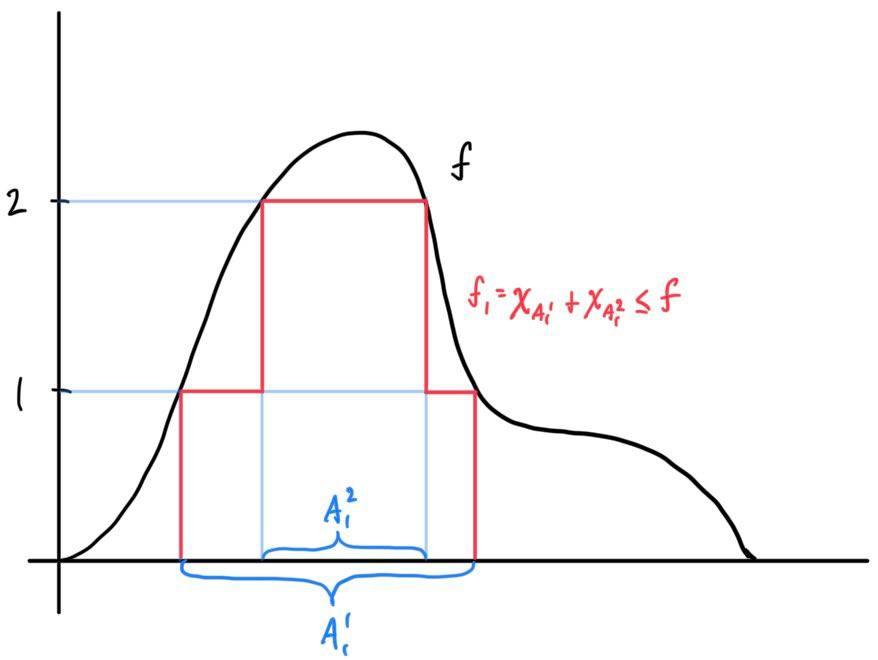
\includegraphics[scale=0.23]{img/Lebesgue_1.jpg}
    \end{center}
    Doing this again with finer subintervals of the codomain gives us, with $f_2 = \chi_{A_2^1} + \chi_{A_2^2} + \chi_{A_2^3} + \chi_{A_2^4} \leq f$. 
    \begin{center}
      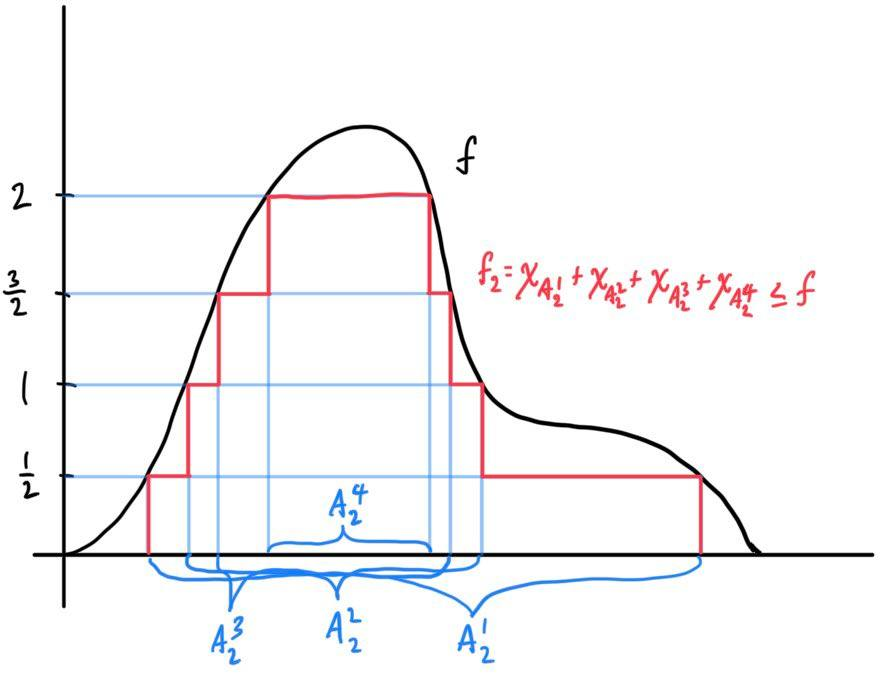
\includegraphics[scale=0.23]{img/Lebesgue_2.jpg}
    \end{center}
    and in general, we have $f_k = \sum_{j=1}^\infty \frac{1}{2^{k-1}} \chi_{A^j_k}$. But we said a simple function is a \textit{finite} sum, and if $\infty$ is in the range of $f$, then this becomes a problem. We can quickly fix this by just truncating the summation at a certain point in the codomain ($f_1$ only considers intervals up to $1$, $f_2$ up to $2$ and so on), ultimately giving us 
    \begin{equation}
      f_k = \sum_{j=1}^{k 2^{k-1}} \frac{1}{2^{k-1}} \chi_{A^j_k} 
    \end{equation}
  \end{proof}


\section{Composing Classes}

  If you find yourself nesting built-in types, this is prob an indicator to compose classes. @dataclass.dataclass operator to define simple data structures. 


\section{Decorators}

  Note that in Python, functions are first-class citizens, which means three things: 
  \begin{enumerate}
    \item They can be treated as objects. 
      \begin{lstlisting}
        def shout(text): 
          return text.upper() 

        print(shout('Hello'))  # HELLO 
        yell = shout 
        print(yell('Hello'))   # HELLO
      \end{lstlisting}
    \item They can be passed into another function as an argument. 
      \begin{lstlisting}
        def shout(text): 
          return text.upper() 

        def whisper(text): 
          return text.lower() 

        def greet(func): 
          greeting = func("Hi, How are You.")
          print (greeting) 

        greet(shout)    # HI, HOW ARE YOU.
        greet(whisper)  # hi, how are you. 
      \end{lstlisting}
    \item They can be returned by another function. 
      \begin{lstlisting}
        def create_adder(x): 
          def adder(y): 
            return x+y 

          return adder 

        add_15 = create_adder(15) 
        print(add_15(10)) # 25 
      \end{lstlisting}
  \end{enumerate}

  Say that you have a function \texttt{f} that does something. I want to modify the behavior so that I do something either before of after \texttt{f} is called automatically, but I don't want to manually add code into the function body. What I can do is simply define another function \texttt{wrapper} and call \texttt{f} inside it. 
  \begin{lstlisting}
    def f(): 
        print("Hello world") 

    def wrapper(): 
        print("started") 
        f()
        print("ended") 

    wrapper() # "started\n Hello world\n ended"
  \end{lstlisting}

  Great, we can do this for one function. But what if there were thousands of functions I want to do this for? Rather than creating a wrapper function for each function, I can make a third function called \texttt{decorator} that takes in the original function \texttt{f} and outputs the \texttt{wrapper} function. 

  \begin{lstlisting}
    def decorator(f): 
      def wrapper(): 
        print("started") 
        f()
        print("ended") 

      return wrapper

    def f(): 
      print("Hello world") 

    wrapper = decorator(f)
    wrapper() # "started\n Hello world\n ended"

    decorator(f) # <function decorator.<locals>.wrapper at 0x100b38e00>
    decorator(f)() # "started\n Hello world\n ended"
  \end{lstlisting}

  This way, I can modify any function I want with this behavior, and is known as \textit{function aliasing}. This is essentially what a decorator is. 

  \begin{definition}[Decorators]
    \textbf{Decorators} are used to modify the behavior of your functions without changing its actual code, used with the \texttt{\@} operator. The two are equivalent. 

    \noindent\begin{minipage}{.5\textwidth}
    \begin{lstlisting}[]{Code}
      def decorator(f): 
        def wrapper(): 
          print("started") 
          f()
          print("ended") 

        return wrapper

      def f(): 
        print("Hello world") 

      f = decorator(f)
      f() # "started\n Hello world\n ended"
    \end{lstlisting}
    \end{minipage}
    \hfill
    \begin{minipage}{.49\textwidth}
    \begin{lstlisting}[]{Output}
      def decorator(f): 
        def wrapper(): 
          print("started") 
          f()
          print("ended") 

        return wrapper

      @decorator
      def f(): 
        print("Hello world") 

      f() # "started\n Hello world\n ended"
    \end{lstlisting}
    \end{minipage}

    This means that every time I call the function \texttt{f}, it really calls the function \texttt{decorator} with \texttt{f} passed into it as an argument. With functions that have arguments, the wrapper function should also have the same arguments. Generically, we can just use the \texttt{\*args} and \texttt{\*\*kwargs} arguments to unpack these variables so that \texttt{wrapper}'s arguments always matches those of \texttt{f}'s arguments, but we can modify these arguments for extra functionality as well. 

    \noindent\begin{minipage}{.5\textwidth}
    \begin{lstlisting}[]{Code}
      # generic args and kwargs
      def decorator(f): 
        def wrapper(*args, **kwargs): 
          print("started") 
          f(*args, **kwargs)
          print("ended") 

        return wrapper

      @decorator
      def f(string): 
        print(string) 

      f("Hello World")
      # started
      # Hello World
      # ended
    \end{lstlisting}
    \end{minipage}
    \hfill
    \begin{minipage}{.49\textwidth}
    \begin{lstlisting}[]{Output}
      # custom arguments 
      def decorator(f): 
        def wrapper(string, start_msg): 
          print(start_msg) 
          f(string)
          print("ended") 

        return wrapper

      @decorator
      def f(string): 
        print(string) 

      f("Hello World", "time to go")
      # time to go
      # Hello World
      # ended
    \end{lstlisting}
    \end{minipage}
    If we want to get the return values of this function, we can store the return value in temporary variable \texttt{tmp}, run whatever code after the function \texttt{f}, and finally return \texttt{tmp} in \texttt{wrapper}. 

    \begin{lstlisting}
      def decorator(f): 
          def wrapper(*args, **kwargs): 
              print("started") 
              tmp = f(*args, **kwargs)
              print("ended") 
              return tmp

          return wrapper

      @decorator
      def f(string): 
          return string + "!"

      print(f("Hello World"))
      # started
      # ended
      # Hello World!
    \end{lstlisting}
  \end{definition}

  \begin{example}[Measuring Total and CPU Runtime]
    If we want to find the runtime of a function, we can do this easily. 

    \begin{lstlisting}
      import time 

      def runtime(f): 
        def wrapper(*args, **kwargs): 
          start = time.time() 
          product = f(*args, **kwargs) 
          end = time.time() 
          print(f"Took {end - start} s") 
          return product
        return wrapper

      @runtime
      def dot(list1, list2): 
        res = 0 
        for x, y in zip(list1, list2): 
          res += x * y 
        return res

      x = [1, 2, 3]
      y = [2, 2, 3]
      result = dot(x, y)  # Took 3.814697265625e-06 s 
      print(result)       # 15 
    \end{lstlisting}

    However, this is not accurate as the OS will switch between different processes. Therefore, the process time is more accurate. 

    \begin{lstlisting}
      import numpy as np
      import time

      def cpu_usage(f):
        def wrapper(*args, **kwargs):
          start_cpu = time.process_time()
          result = f(*args, **kwargs)
          end_cpu = time.process_time()
          print(f"CPU time: {end_cpu - start_cpu:.6f} seconds")
          return result
        return wrapper

      @cpu_usage
      def matrix_mult(a, b): 
        return np.matmul(a, b)

      x = np.random.randn(2000, 2000)

      matrix_mult(x, x) # CPU time: 0.772730 seconds
    \end{lstlisting}
  \end{example}

  \begin{example}[Memory Usage]
    We can measure memory usage with the \texttt{psutil} library. 
    \begin{lstlisting}
      import numpy as np
      import psutil, os 

      def memory_usage(f):
        def wrapper(*args, **kwargs):
          process = psutil.Process(os.getpid())
          mem_before = process.memory_info().rss
          result = f(*args, **kwargs)
          mem_after = process.memory_info().rss
          print(f"Memory usage: {(mem_after - mem_before) / 1024 / 1024:.2f} MB")
          return result
        return wrapper

      @memory_usage 
      def matrix_mult(a, b): 
        return np.matmul(a, b)

      x = np.random.randn(2000, 2000)
      matrix_mult(x, x) # Memory usage: 46.81 MB
    \end{lstlisting}
  \end{example}

  \begin{example}[Measuring Function Call Count]
    To measure how many times a function has been called, we can use the decorator. 
    \begin{lstlisting}
      def call_counter(f):
          def wrapper(*args, **kwargs):
              wrapper.count += 1
              print(f"Function '{f.__name__}' called {wrapper.count} times")
              return f(*args, **kwargs)
          wrapper.count = 0
          return wrapper

      @call_counter
      def factorial(x): 
          if x == 1: 
              return 1 
          return x * factorial(x - 1)

      result = factorial(7)
      # Function 'factorial' called 1 times
      # Function 'factorial' called 2 times
      # Function 'factorial' called 3 times
      # Function 'factorial' called 4 times
      # Function 'factorial' called 5 times
      # Function 'factorial' called 6 times
      # Function 'factorial' called 7 times
      print(result)       
      # 5040
    \end{lstlisting}
  \end{example}

  functools.wraps. 


\section{Raising Exceptions}

  Many beginners prefer to return None, but you should really be raising exceptions. 


\section{Package Management}



\section{Inspect} 

  \texttt{inspect} is a module that allows you to get live information about live objects such as modules, classes, and functions. 

  
  \begin{definition}[\texttt{getsource}]
    The \texttt{getsource} method allows you to see the text of live objects. 

    \begin{figure}[H]
      \centering 
      \begin{lstlisting}
        >>> import inspect 
        >>> backbone_module = construct_backbone('resnet50[pretraining=inaturalist]')
        >>> model = backbone_module.embedded_model 
        >>> print(inspect.getsource(model.forward))
            def forward(self, x):
                x = self.conv1(x)
                x = self.bn1(x)
                x = self.relu(x)
                x = self.maxpool(x)

                x = self.layer1(x)
                x = self.layer2(x)
                x = self.layer3(x)
                x = self.layer4(x)

                return x

        >>> print(inspect.getsource(model.__class__))
        class ResNet_features(nn.Module):
            """
            the convolutional layers of ResNet
            the average pooling and final fully convolutional layer is removed
            """

            def __init__(self, block, layers, num_classes=1000, zero_init_residual=False):
                super(ResNet_features, self).__init__()
                ...
            ...
      \end{lstlisting}
      \caption{Say that you have some torch model that is either inaccessible or is hidden away through so many imports that you have a hard time accessing it. Rather than going through several files and having to parse which methods are relevant, is overwritten, or called, you can just inspect the methods and classes directly.}
    \end{figure}
  \end{definition}

 
\end{document}
